%%%%%%%%%%%%%%%%%%%%%%%%%%%%%%%%%%%%%%%%%%%%%%%%%%%%%%%%%%%
% --------------------------------------------------------
% EPFL QSE: Semester Project Documentation
% 
% Authors: 
% Cherilyn Lee Gabriela Christen,
% Nathaniel James Pacey
% 
% License:
% Creative Commons CC BY 4.0
% --------------------------------------------------------
%%%%%%%%%%%%%%%%%%%%%%%%%%%%%%%%%%%%%%%%%%%%%%%%%%%%%%%%%%%

\documentclass[9pt,a4paper,twocolumn,twoside]{tau-class/tau}
\usepackage{parskip}  
\setlength{\parskip}{0.5em}     % Small space between paragraphs
\setlength{\parindent}{0pt}     % No paragraph indentation
% Reduce vertical space around equations
\setlength{\abovedisplayskip}{0pt}
\setlength{\belowdisplayskip}{0pt}
\setlength{\abovedisplayshortskip}{0pt}
\setlength{\belowdisplayshortskip}{0pt}
\setlength{\textfloatsep}{8pt}
\setlength{\floatsep}{6pt}
\setlength{\intextsep}{6pt}


\usepackage[english]{babel}
\usepackage{graphicx} % Required for inserting images
\usepackage{algpseudocode}
\usepackage{graphicx} % Required for inserting images
\usepackage{xcolor}
\usepackage{graphicx}
\usepackage{multicol}
\usepackage{braket}
\usepackage{enumitem}
\usepackage{tikz}
\usepackage{quantikz}
\usepackage{hyperref}



%----------------------------------------------------------
% Effect of Stochastic Noise on Surface Codes
%----------------------------------------------------------

\title{Effect of Stochastic Gate Noise on Fault-Tolerant Surface Codes}

%----------------------------------------------------------
% AUTHORS, AFFILIATIONS AND PROFESSOR
%----------------------------------------------------------

\author[b,2]{Cherilyn Lee Gabriela Christen, Nathaniel James Pacey}


%----------------------------------------------------------

\professor{In work under EPFL supervising Professor. Nicolas Macris}

%----------------------------------------------------------
% FOOTER INFORMATION
%----------------------------------------------------------

\institution{EPFL}
\footinfo{\LaTeX\ Template}
\theday{April 15, 2025}
\leadauthor{Christen, Pacey.}
\course{EPFL QSE}


%----------------------------------------------------------

\keywords{\LaTeX\ class, lab report, academic article, tau class}
\begin{document}
\maketitle
%----------------------------------------------------------
\section{Abstract}
This work investigates the effects of physically motivated single-qubit stochastic noise on quantum circuits. We simulate this noise in surface code layouts to better understand and improve error mitigation. Following the surface code layouts introduced by Fowler et al. we reproduced both a 4-qubit and 9-qubit version of the planar code using Qiskit~\cite{fowler2012surface}. To introduce realistic noise, we integrated and extended the noisy gates framework developed by Di Bartolomeo et al. adapting it to support arbitrary-axis single-qubit rotations (\( R_{xyz} \)) and additional functionality such as mid-circuit measurements and noisy reset operations~\cite{dibartolomeo2023noisy}.

To analyze the stochastic noise model in detail, we implemented the 4-qubit surface code in QuTiP, allowing direct evaluation of stabilizer outcomes and quantitative noise properties such as fidelity, trace preservation, and Hellinger distance. These simulations matched expected behavior and aligned with Qiskit’s noisy simulator results, offering preliminary validation of the noise model. Though full error correction and two-qubit noise are not yet included, this work establishes a foundation for simulating logical qubits and evaluating their stability; key steps toward benchmarking and refining error mitigation on real quantum hardware.


\section{Motivation}
Quantum computers offer the potential to solve certain problems, like unstructured search or integer factorization, exponentially faster than classical computers, where such tasks remain computationally intensive~\cite{ncbiQuantumOverview2019}. 
Despite active research into various hardware platforms, all current implementations remain limited by noise, decoherence, and operational errors, preventing reliable large-scale computation~\cite{ncbiQuantumOverview2019,fowler2014scalable}.
To overcome these limitations, it is possible to construct logical qubits from multiple noisy physical qubits in such a way that the logical qubit exhibits improved stability and coherence. One of the most powerful frameworks for enabling this kind of error correction is the theory of stabilizer codes, which uses structured sets of commuting Pauli operators to detect and correct errors without collapsing the encoded quantum information \cite{fowler2012surface}. 


\section{Stabilizer Code}
Stabilizer codes define a subspace of the $n$-qubit Hilbert space as the simultaneous +1 eigenspace of an abelian subgroup $\mathcal{S} \subset \mathcal{P}_n$, where $\mathcal{P}_n$ is the $n$-qubit Pauli group \cite{gottesman1997stabilizer}. A stabilizer code that encodes $k$ logical qubits into $n$ physical qubits is specified by $n - k$ independent generators $\{ S_1, \dots, S_{n-k} \} \in \mathcal{P}_n$, each satisfying $S_i^2 = I$ and $[S_i, S_j] = 0$ \cite{gottesman1997stabilizer}. The code space is the set of states $|\psi\rangle$ such that $S_i |\psi\rangle = |\psi\rangle$ for all $i$. Logical operators commute with all elements of $\mathcal{S}$ but are not themselves in $\mathcal{S}$ \cite{gottesman1997stabilizer}.

To see how stabilizer codes detect errors, consider what happens when a Pauli error $E$ acts on a valid codeword $|\psi\rangle$, which satisfies $S|\psi\rangle = |\psi\rangle$ for all $S \in \mathcal{S}$. Now consider measuring a stabilizer generator \( S_i \) after the error:
\begin{equation}
    S_i(E|\psi\rangle) = \pm E S_i |\psi\rangle = \pm E |\psi\rangle
    \label{eq: stabilizer}
\end{equation}
\begin{itemize}[left=0pt]
    \item If \( E \) \textit{commutes} with \( S_i \): \( S_i(E|\psi\rangle) = E|\psi\rangle \) $\rightarrow$ you get a +1 measurement, same as if no error happened — the error is undetectable by that stabilizer.
    \item If \( E \) \textit{anticommutes} with \( S_i \): \( S_i(E|\psi\rangle) = -E|\psi\rangle \) $\rightarrow$ you get a -1 measurement - the syndrome detects a change.
\end{itemize}
This formalism provides a compact and scalable way to describe quantum codes and is the basis for surface codes \cite{fowler2012surface}.

\section{Surface Code}
The surface code is a topological stabilizer code defined on a 2D lattice, where qubits are placed on the edges of a square grid. These are the data qubits, which hold the encoded quantum information. In addition, the code includes measurement qubits (or ancilla qubits), each responsible for extracting error syndromes by measuring stabilizer operators. Every measurement qubit is entangled with its four neighboring data qubits during the stabilizer circuit and implements either a measure-X or measure-Z operator, detecting bit-flip or phase-flip errors, respectively. Each data qubit is coupled to two measure-Z and two measure-X qubits, allowing full syndrome coverage of possible single-qubit errors \cite{fowler2012surface}.

\subsection{Cycles and Quiescent States}
Surface code operation proceeds in repeated measurement cycles; during which each measure-Z and measure-X qubit performs a stabilizer measurement on its four neighboring data qubits. For a Z-stabilizer in a 4-qubit surface code, this involves applying four CNOT gates with the data qubits as controls and the measurement qubit as target, projecting the data into an eigenstate of $Z_a Z_b Z_c Z_d$. Here, $Z_a Z_b Z_c Z_d$ represents the tensor product of Pauli-Z operators acting on the four data qubits surrounding the Z-type measurement qubit. The X-stabilizers follow the same structure but include Hadamard gates before and after the CNOTs\footnote{By \( H Z H = X \), Hadamards convert a \( Z \)-basis measurement into an \( X \)-basis measurement.}, effectively measuring $X_a X_b X_c X_d$, where each $X_i$ acts on a neighboring data qubit around the corresponding X-type measurement qubit. Once all stabilizer measurements are complete, the data qubits are projected into a state that simultaneously satisfies all measured eigenvalue constraints, this is known as the quiescent state \cite{fowler2012surface}. 

Importantly, stabilizer codes do not operate from a fixed ground state but from one of exponentially many possible quiescent states, each defined by the outcomes of the stabilizer measurements. These cycles are repeated, and in the absence of errors, the quiescent state remains stable due to the commutation of all stabilizers. 

\subsection{Errors}
One of the key features of the surface code is its focus on error detection rather than direct error correction. Physical corrections are only applied if an error affects a measurement outcome; otherwise, errors are tracked in software using the surface code’s classical decoder and effectively neutralize themselves when they reoccur in the same way.


While implementing a single logical qubit in a non-rotated surface code requires a minimum of 13 physical (data) qubits, achieving a reasonably fault-tolerant logical qubit suitable for practical quantum computation typically demands on the order of $10^3$ to $10^4$ physical qubits. This number depends strongly on the rate that errors occur on the physical qubits \cite{fowler2012surface}. 

\begin{figure}[htbp]
    \centering
    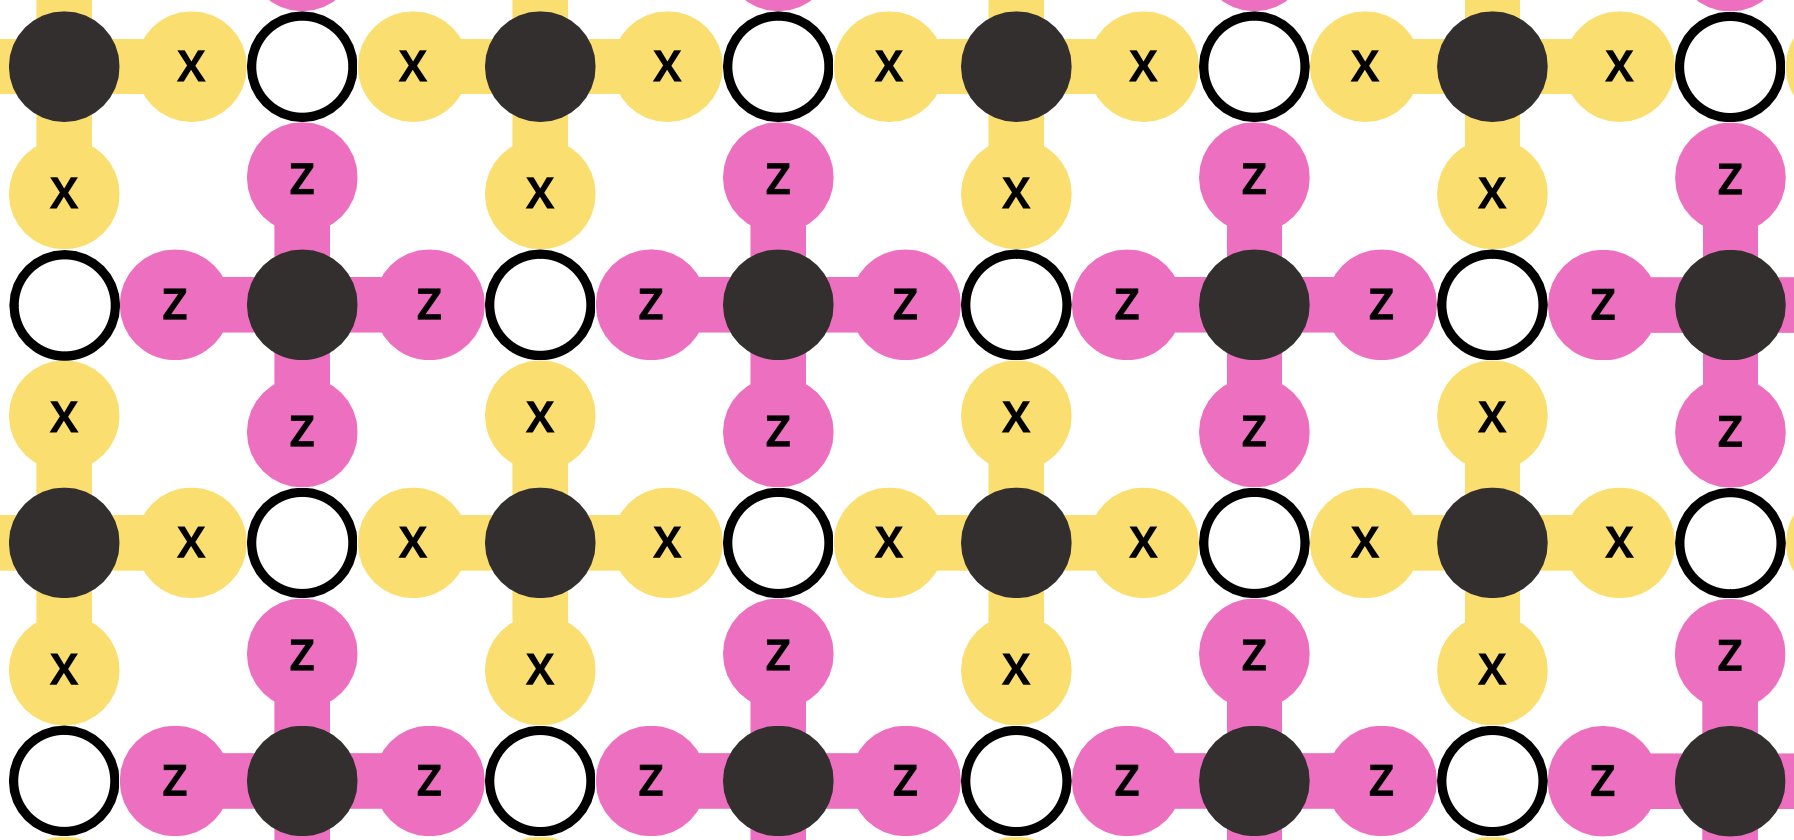
\includegraphics[width=0.35\textwidth]{figures/Surface Code Example.png}
    \caption{Layout of a surface code lattice. White circles represent data qubits, yellow (X) and pink (Z) are measurement qubits. Each measurement qubit is entangled with its four neighboring data qubits and measures either an X-type or Z-type stabilizer.}
    \label{fig:layout}
\end{figure}

\subsection{Logical Qubit}
A logical qubit in the surface code is defined using the degrees of freedom that remain after imposing all stabilizer constraints. In a 2D surface code array, these constraints typically do not fully determine the quantum state due to the presence of topological boundaries \cite{fowler2012surface}. For instance, in a square surface with 41 data qubits and only 40 independent $\hat{X}$ and $\hat{Z}$ stabilizers, there remain two unconstrained degrees of freedom, sufficient to encode a single logical qubit. Logical operators $\hat{X}_L$ and $\hat{Z}_L$ are constructed as products of single-qubit Pauli operators that commute with all stabilizers but are not themselves stabilizers. In the configuration shown in Fig.~\ref{fig:Logical Qubit}, a logical $\hat{X}_L$ operator is defined as $\hat{X}_L = \hat{X}_1 \hat{X}_2 \hat{X}_3 \hat{X}_4 \hat{X}_5$, forming a string that connects the two smooth (X-type) boundaries. A corresponding logical $\hat{Z}_L$ operator connects the rough (Z-type) boundaries and is defined as $\hat{Z}_L = \hat{Z}_1 \hat{Z}_2 \hat{Z}_3 \hat{Z}_4 \hat{Z}_5$. Both operators commute with all stabilizers and anticommute with each other, satisfying $\hat{X}_L \hat{Z}_L = -\hat{Z}_L \hat{X}_L$, just like physical Pauli operators. Applying $\hat{X}_L$ or $\hat{Z}_L$ to the quiescent state $|\psi\rangle$ results in new code states $|\psi_X\rangle = \hat{X}_L |\psi\rangle$ or $|\psi_Z\rangle = \hat{Z}_L |\psi\rangle$, which share the same stabilizer measurement outcomes as $|\psi\rangle$, but differ by a logical bit or phase flip. Alternative logical operators, such as $\hat{X}'_L = \hat{X}_1 \hat{X}_{11} \hat{X}_{12} \hat{X}_{13} \hat{X}_3 \hat{X}_4 \hat{X}_5$, differ from $\hat{X}_L$ by a product of stabilizers and act identically on the code space, up to an eigenvalue determined by the stabilizer measurement outcome \cite{fowler2012surface}. Thus, all logical operators that implement the same logical transformation form an equivalence class modulo the stabilizer group, and only the representative modulo stabilizers, like $\hat{X}_L$ and $\hat{Z}_L$, are needed to define the encoded logical qubit \cite{fowler2012surface}.

\begin{figure}[htbp]
    \centering
    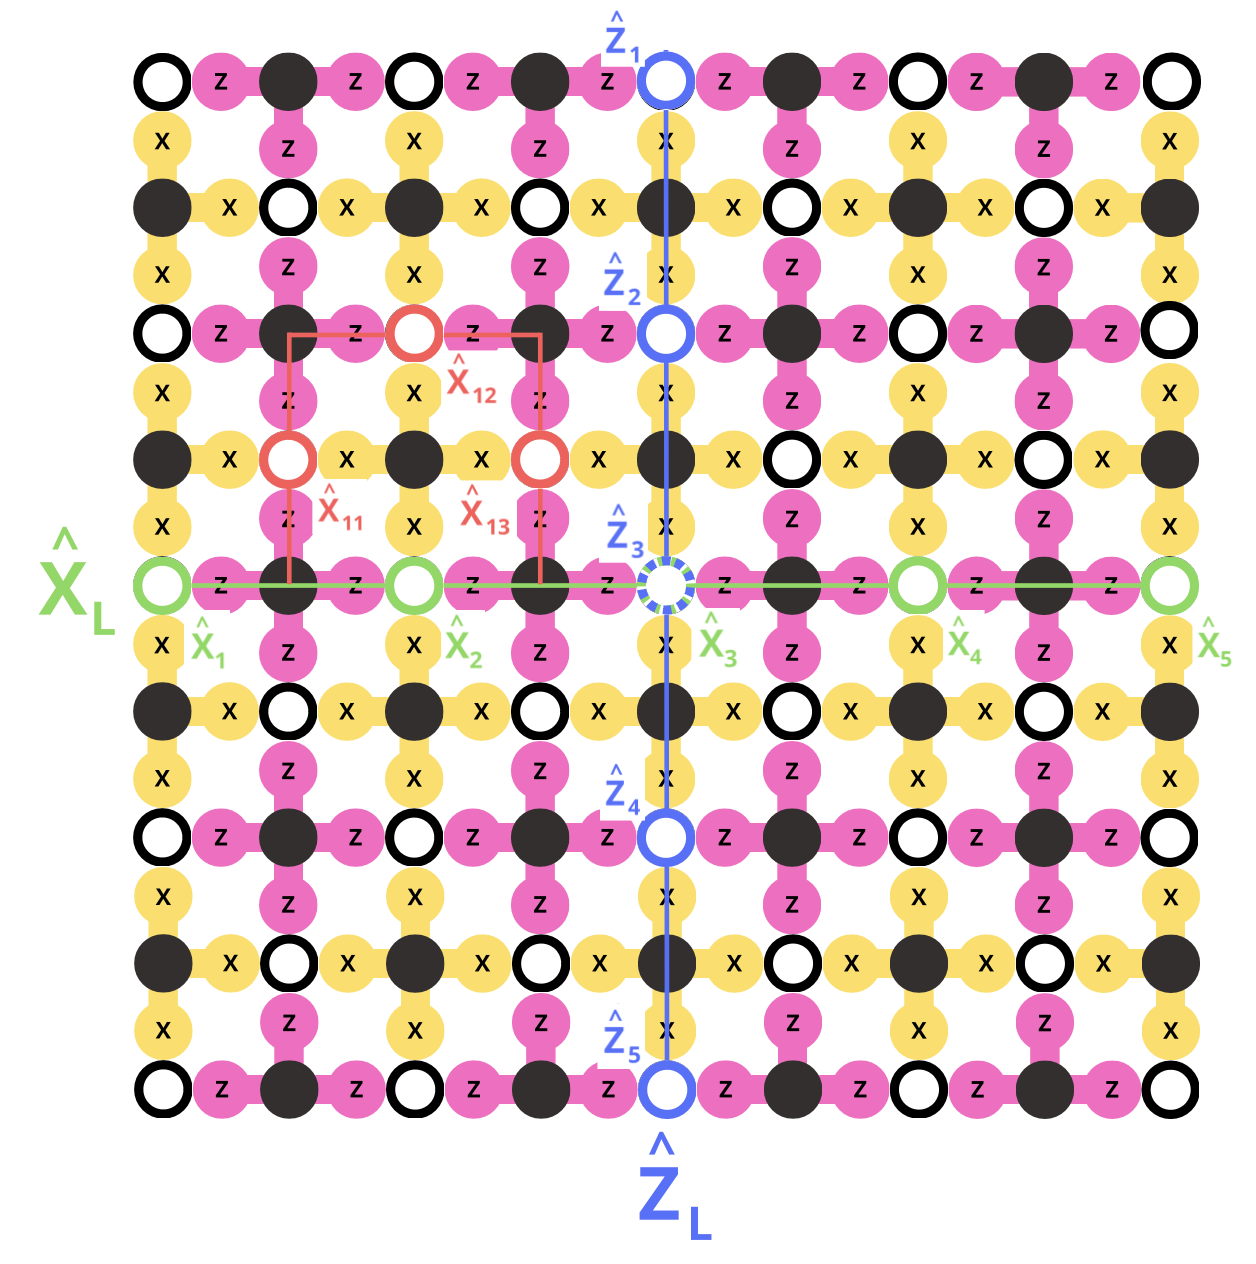
\includegraphics[width=0.4\textwidth]{figures/Logical Qubit.png}
    \caption{Surface code layout showing logical operators $\hat{X}_L$ (green) and $\hat{Z}_L$ (blue) as strings of Pauli operators spanning the lattice between opposite boundaries \cite{fowler2012surface}.}
    \label{fig:Logical Qubit}
\end{figure}

To illustrate the structure of a logical qubit in the surface code, we consider a minimal working example consisting of 9 physical qubits: 5 data qubits and 4 measurement qubits. This layout defines a surface code with four independent stabilizers, leaving $(5_{\text{data qubits}} - 4_{\text{stabilizers}}) \times 2 = 2_{dof}$, unconstrained degrees of freedom, sufficient in principle, to encode a single logical qubit. However, this configuration lacks sufficient code distance to correct arbitrary single-qubit errors. To achieve minimum-distance error correction (i.e., robustness to any single-qubit error), the layout must be extended. In the rotated surface code, this requires 9 data qubits and 8 ancilla qubits (17 physical qubits in total) \cite{fowler2014scalable}. Alternatively, in the non-rotated surface code considered by Fowler, a distance-3 code requires 13 data qubits and 12 measurement qubits, totaling 25 physical qubits for a fully fault-tolerant logical qubit~\cite{fowler2012surface}.

\section*{4 Qubit Example}
In this example, we consider 4 qubits, 2 measurement qubits and 2 data qubits. We note that this particular structure does not give rise to a logical qubit since there is no additional degree of freedom to be extracted from the structure. It is instead meant as an example to better understand the workings of the surface code.
We assume the two data qubits $D_a$ and $D_b$ in a general state, 
\begin{equation}
    \ket{\psi}_{a,b}=A\ket{gg}+B\ket{ge}+C\ket{eg}+D\ket{ee}.
    \label{eq: general state 2 qubits}
\end{equation}
with \(|A|^2 + |B|^2+|C|^2+|D|^2 = 1\). Wether this is an entangled or a product state doesn't change the process. 
The measurement qubits $M_x$ and $M_z$ are both initialized to the ground state $\ket{g}$ \cite{fowler2012surface}. The complete initial state is: 
\begin{align}
    \ket{\psi_0} &= \ket{g} \otimes \ket{\psi}_{a,b} \otimes \ket{g}\notag \\
    &= A\ket{gggg}+B\ket{ggeg}+C\ket{gegg}+D\ket{geeg} 
    \label{eq: general state 4 qubits}
\end{align}

\vspace{-\baselineskip}
\begin{figure}[ht]
% Subfigure (a)
\begin{subfigure}[b]{0.17\textwidth}
    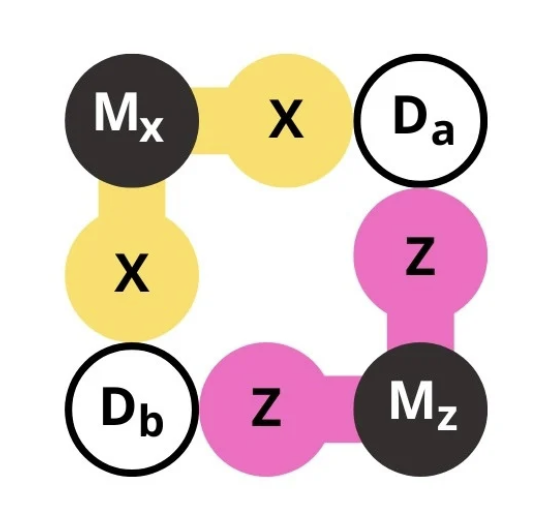
\includegraphics[scale=0.3]{figures/4 qubits.jpeg}
\end{subfigure}
% Subfigure (b)
\raisebox{3.7em}{ % manually adjust height to align with circuit
\begin{subfigure}[b]{0.29\textwidth}
    \scalebox{0.7}{
    \begin{quantikz}[row sep=0.2cm, column sep=0.4cm]
    \lstick{$\textbf{$M_x$}$} & \push{\ket{g}}\qw  & \gate{H} & \ctrl{1} & \ctrl{2} & \qw      & \qw      & \gate{H} & \meter{} & \qw\\
    \lstick{$D_a$}          & \qw                & \gate{I} & \targ{}  & \qw      & \ctrl{2} & \qw      & \gate{I} & \qw & \qw\\
    \lstick{$D_b$}          & \qw                & \gate{I} & \qw      & \targ{}  & \qw      & \ctrl{1} & \gate{I} & \qw& \qw \\
    \lstick{$\textbf{$M_z$}$} & \push{\ket{g}}\qw & \gate{I} & \qw      & \qw      & \targ{}  & \targ{}  & \gate{I} & \meter{}& \qw
    \end{quantikz}
    }
\end{subfigure}}
\caption{(a) and (b): Layout and circuit for stabilizer measurements \cite{fowler2012surface}.}
\label{fig:combined}
\end{figure}

\textbf{Step 1: } Apply the Hadamard gate to the X measurement qubit to change the basis \cite{fowler2012surface}. 
\begin{align}
\ket{\psi_1} &= H_{M_x} I_{D_a} I_{D_b} I_{M_z}\ket{\psi_0} = (\ket{g} + \ket{e}) \otimes \ket{\psi}_{a,b} \otimes \ket{g}
\label{eq: step 1}
\end{align}
\textbf{Step 2: }
Apply the CNOT gates to create the entangled states \cite{fowler2012surface}. 
\begin{align} 
\ket{\psi_2} &= CNOT_{M_x \rightarrow D_a} CNOT_{M_x \rightarrow D_b} CNOT_{D_a \rightarrow M_z} CNOT_{D_b \rightarrow M_z}\ket{\psi_1} \notag\\ &=
A(\ket{gggg}+ \ket{eeeg}) +B(\ket{ggee}+\ket{eege}) \notag\\ &+C(\ket{gege}+\ket{egee} ) +D(\ket{geeg}+ \ket{eggg})
\label{eq: step 2}
\end{align}
\textbf{Step 3: } 
Apply the Hadamard gate to the X measurement qubit to change the basis back to the Z basis to be able to conduct a measurement in the Z basis \cite{fowler2012surface}. 
\begin{align}
    \ket{\psi_3} 
    &= H_{M_x} I_{D_a} I_{D_b} I_{M_z}\ket{\psi_2} \notag \\
    &=A(\ket{gggg} + \ket{eggg} + \ket{geeg} - \ket{eeeg}) \notag \\ 
    &+B(\ket{ggee} + \ket{egee} + \ket{gege} - \ket{eege}) \notag\\
    &+C(\ket{gege} + \ket{eege} + \ket{ggee} - \ket{egee}) \notag\\
    &+D(\ket{geeg} + \ket{eeeg} + \ket{gggg} - \ket{eggg})
    \label{eq: step 3a}
\end{align}
\begin{align}
    \ket{\psi_3}   
    &=(A+D)(\ket{g}_{M_x} \otimes (\ket{gg}+\ket{ee})_{D_a,D_b} \otimes \ket{g}_{M_z}) \notag\\
    &+(B+C)(\ket{g}_{M_x} \otimes (\ket{ge}+\ket{eg})_{D_a,D_b} \otimes \ket{e}_{M_z}) \notag\\
    &+(A-D)(\ket{e}_{M_x} \otimes (\ket{gg}-\ket{ee})_{D_a,D_b} \otimes \ket{g}_{M_z}) \notag\\
    &+(B-C)(\ket{e}_{M_x} \otimes (\ket{ge}-\ket{eg})_{D_a,D_b} \otimes \ket{e}_{M_z})
    \label{eq: step 3b}
\end{align}
Here it becomes obvious that the quiescent states of $D_a$ and $D_b$ are the bell states. It can be deducted in which quiescent state $D_a$ and $D_b$ are, based on the measurement outcome on the qubits $M_x$ and $M_z$. In the subsequent cycles, on a perfect circuit (no errors occurring) the quiescent state will stay constant \cite{fowler2012surface}. For Example, if the measurement on the $M_x$ and $M_z$ qubits results in a {+1,+1} then the data qubits are in state $\ket{B_{00}}$. This implies $A=D=\frac{1}{\sqrt{2}},$ and $ B = C = 0$ for $\ket{\psi_0}$ in the next cycle. Therefore, $\ket{\psi_3} = (\ket{g}_{M_x} \otimes (\ket{gg}+\ket{ee})_{D_a,D_b} \otimes \ket{g}_{M_z})$ with probability 1. 

\subsection{Error Detection}
Now we will analyse the impact of certain, simple gate errors in the circuit. For this example we will focus on the impact of having a Pauli gate instead of an Identity gate on the data qubit as seen in Fig.~\ref{fig:quantum circuit 4 qubits}. Assuming the quiescent state of $D_a$ and $D_b$ has been determined in the first cycle, it is expected to stay constant over the next cycles given that no error occurs. A Pauli-$X$ error on the data qubit anticommutes with the $Z$-type stabilizer $M_z$, and thus will be detected as a change in the corresponding measurement outcome. Conversely, a Pauli-$Z$ error anticommutes with the $X$-type stabilizer $M_x$ and is similarly flagged by a measurement flip \cite{fowler2012surface}. 
\begin{figure}[ht]
\centering
\scalebox{0.7}{  % Adjust scale as desired
\begin{quantikz}[row sep=0.2cm, column sep=0.4cm]
\lstick{$\textbf{$M_x$}$} & \push{\ket{g}}\qw  & \gate{H} & \ctrl{1} & \ctrl{2} & \qw      & \qw      & \gate{H} & \meter{} & \qw\\
\lstick{$D_a$}          & \qw                & \gate[style={fill=red!30}]{?}  & \targ{}  & \qw      & \ctrl{2} & \qw      & \gate{I} & \qw & \qw\\
\lstick{$D_b$}          & \qw                & \gate{I} & \qw      & \targ{}  & \qw      & \ctrl{1} & \gate{I} & \qw & \qw\\
\lstick{$\textbf{$M_z$}$} & \push{\ket{g}}\qw & \gate{I} & \qw      & \qw      & \targ{}  & \targ{}  & \gate{I} & \meter{}& \qw
\end{quantikz}
}
\caption{Quantum circuit on 4 qubits with gate error on the red gate.}
\label{fig:quantum circuit 4 qubits}
\end{figure}
\subsubsection*{X-Error}
If a X-error occurs on the $D_a$ qubit the state on $D_a$ and $D_b$ is  $\ket{\psi}_{D_a,D_b}=\ket{eg} + \ket{ge}$ and no longer $\ket{\psi}_{D_a,D_b}=\ket{gg} + \ket{ee}$ (neglecting normalization coefficents). This implies $A=D=0$ and $B = C = 1$ which means the only non-zero coefficient in $\ket{\psi_3}$ is \(\ket{g}_{M_x} \otimes (\ket{ge}+\ket{eg})_{D_a,D_b} \otimes \ket{e}_{M_z}\). During the measurements in this cycle, the results will be \{+1,-1\} indicating the occurrence of an X-error. Note that the occurence of two X-errors would cancel out and the measurement results would again be \{+1,+1\} corresponding to the original quiescent state. Similarly if a second X-error occurs on the data qubit $D_b$, $\ket{\psi}_{D_a,D_b}=\ket{ee} + \ket{gg}$, no error will be detected since the quiescent state has not changed from the last cycle. 
\subsubsection*{Z-Error}
Similar reasoning will show the resulting state in the case of a Z-error. A Z-error changes the quiescent state as follows, $\ket{\psi}_{D_a,D_b}=\ket{gg} - \ket{ee} \rightarrow A=-D=1$ and $B=C=0$. Therefore, $\ket{\psi_3}$ is $\ket{e}_{M_x} \otimes (\ket{gg}-\ket{ee})_{D_a,D_b} \otimes \ket{g}_{M_z}$ with measurement outcomes $\{-1,+1\}$. This indicates the occurrence of a Z-error. Again, note that a second Z error on the same qubit or on the other data qubit will cancel out the error and keep the quiescent gate constant. 
\subsubsection*{Y-Error}
A Y-error is a concatenation of X and Z errors, meaning it applies both a bit-flip and a phase-flip to the qubit. The error affects the quiescent state as follows: $\ket{\psi}_{D_a,D_b} = -\ket{eg} + \ket{ge}$ implying $A=D=0$ and $B=-C=1$ which leaves $\ket{\psi_3}$ in state $(\ket{e}_{M_x} \otimes (\ket{ge}-\ket{eg})_{D_a,D_b} \otimes \ket{e}_{M_z})$ with measurement outcomes \{-1,-1\} indicating the Y-Error. 
\subsection{4-Qubit Simulation}
To investigate the impact of gate errors on a quantum stabilizer circuit, we simulated the above discussed 4-qubit system. In the plot in Fig.~\ref{fig:eigenvallues4qubtswitherror}, a measurement value of 0 corresponds to eigenvalue $+1$, and a value of 1 corresponds to eigenvalue $-1$. This is because stabilizer measurements return a binary outcome, where 0 indicates no detected change (i.e., the state is in the $+1$ eigenspace of the stabilizer operator), and 1 indicates a sign flip (i.e., projection onto the $-1$ eigenspace).
\begin{figure}[htbp]
    \centering
    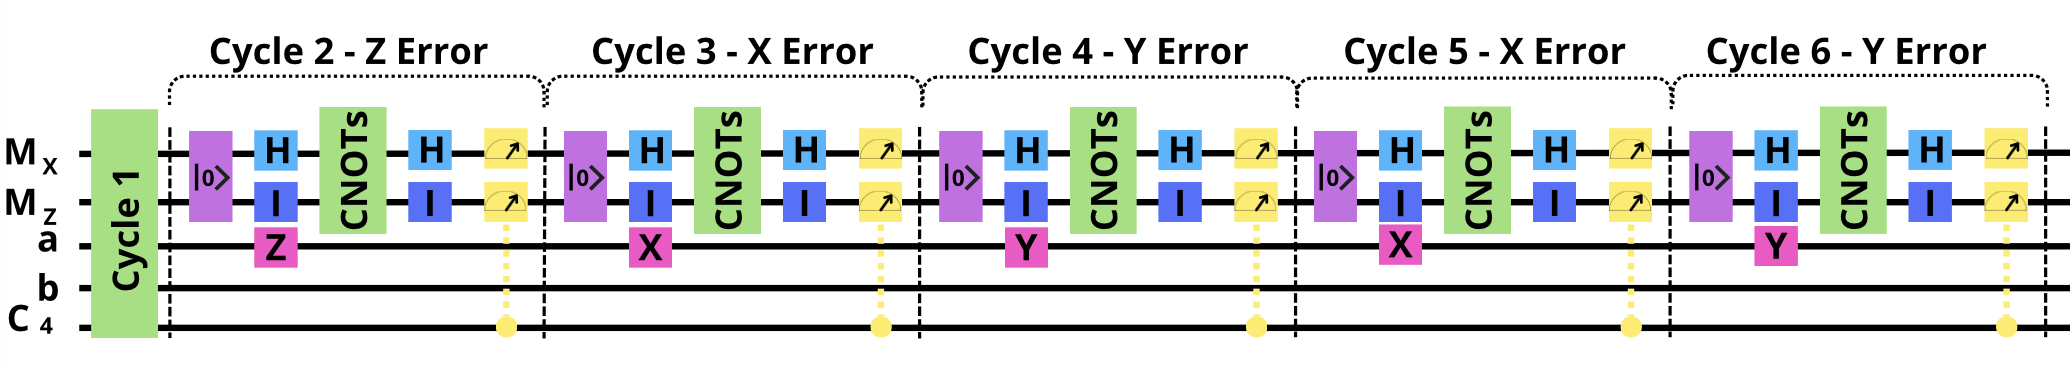
\includegraphics[width=0.48\textwidth]{figures/Circuit4qubitsErrors.png}
    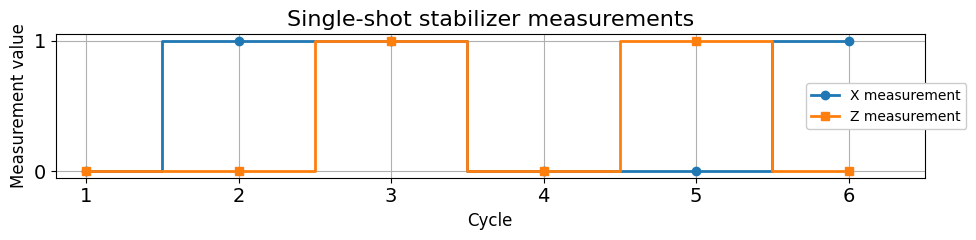
\includegraphics[width=0.48\textwidth]{figures/EigenvaluePlot4qubitsErrors.png}
    \caption{Single-shot stabilizer measurement over 6 cycles on the 4-qubit surface. Here, 0 corresponds to eigenvalue $+1$, and 1 to eigenvalue $-1$.}
    \label{fig:eigenvallues4qubtswitherror}
\end{figure}

The setup is designed to measure both \(X\) and \(Z\) stabilizers in a repetitive manner across six cycles. To model noise, we introduced deliberate single-qubit gate errors, replacing identity gates with \(X\), \(Y\), or \(Z\) gates. The resulting changes in stabilizer eigenvalues were tracked over time. \\
As shown in the eigenvalue plot, a \(Z\) error introduced in cycle 2 causes the eigenvalue of the \(X\) stabilizer to flip from 0 to 1. Subsequently, an \(X\) error in cycle 3 flips the \(Z\) stabilizer’s eigenvalue. In cycle 4, a \(Y\) error (which is equivalent to a combination of \(X\) and \(Z\) errors), reverses both eigenvalues back to 0. Another \(X\) error in cycle 5 causes the \(Z\) stabilizer to flip again, and finally, a \(Y\) error in cycle 6 flips the \(X\) stabilizer back to 0 while putting the \(Z\) stabilizer to 1. These results illustrate how specific error types influence the respective eigenvalue trajectories.
\section*{9 Qubit Example}
\begin{figure}[ht]
% Subfigure (a)
\begin{subfigure}[b]{0.15\textwidth}
    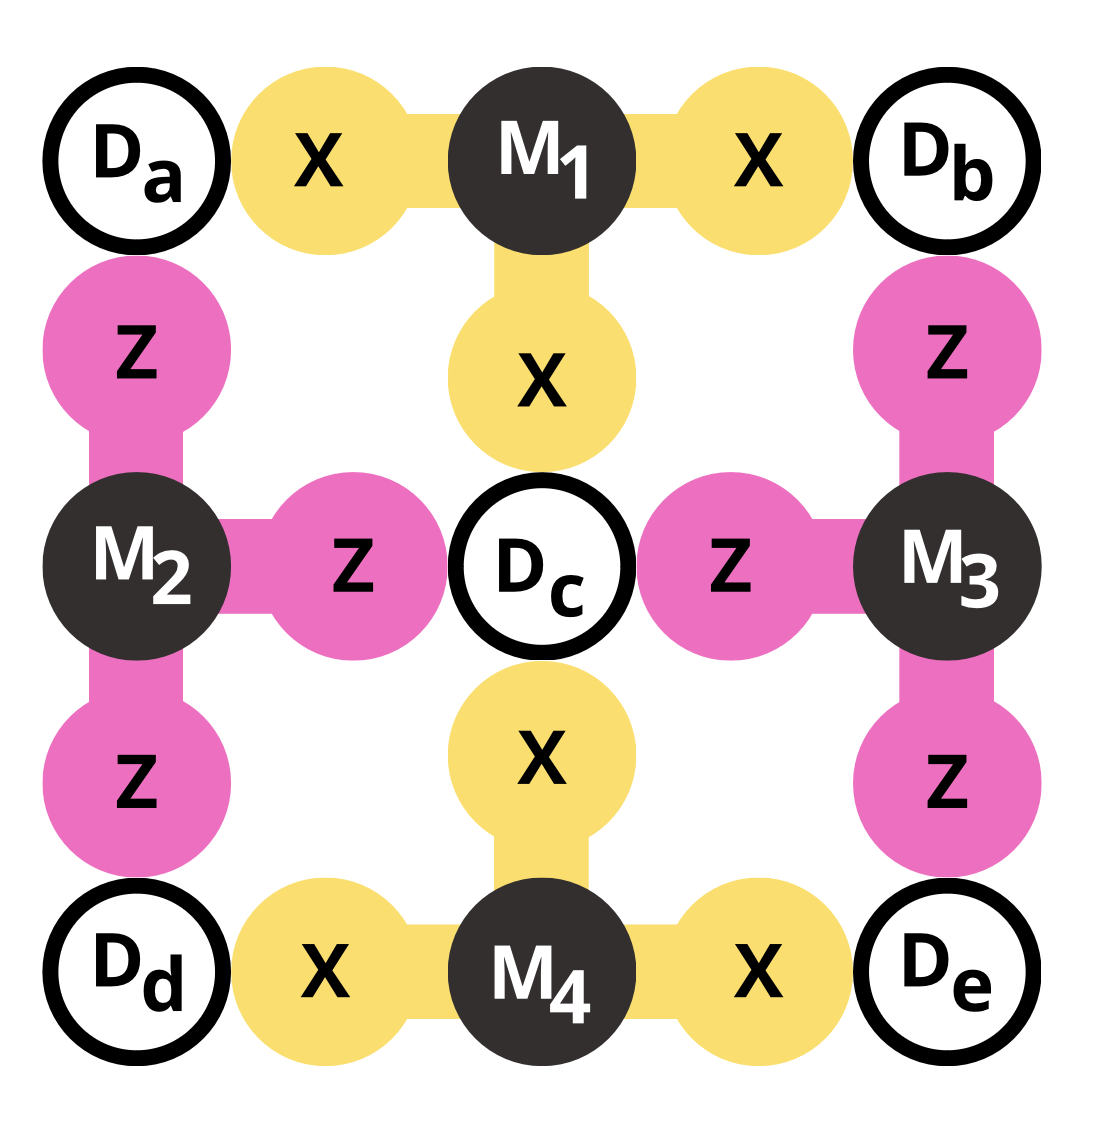
\includegraphics[scale=0.15]{figures/Surface Code Example 9.png}
\end{subfigure}
% Subfigure (b)
\raisebox{4.6em}{ % manually adjust height to align with circuit
\begin{subfigure}[b]{0.2\textwidth}
    \scalebox{0.7}{
    \begin{quantikz}[row sep=0.05cm, column sep=0.1cm]
    \lstick{$M_{X1}$} & \push{\ket{g}} & \gate{H} & \ctrl{4} & \ctrl{5} & \ctrl{6} & \qw      & \qw      & \qw       & \qw      & \qw       & \qw      & \qw       & \qw       & \qw & \gate{H} & \meter{}& \qw\\
    \lstick{$M_{X2}$} & \push{\ket{g}} & \gate{H} & \qw      & \qw      & \qw      & \ctrl{5} & \ctrl{6} & \ctrl{7}  & \qw      & \qw       & \qw      & \qw       & \qw       & \qw & \gate{H} & \meter{}& \qw\\
    \lstick{$M_{Z1}$} & \push{\ket{g}} & \gate{I} & \qw      & \qw      & \qw      & \qw      & \qw      & \qw       & \targ{}  & \targ{}   & \targ{}  & \qw       & \qw       & \qw & \gate{I} & \meter{}& \qw\\
    \lstick{$M_{Z2}$}&  \push{\ket{g}} & \gate{I} & \qw      & \qw      & \qw      & \qw      & \qw      & \qw       & \qw      & \qw       & \qw      & \targ{}   & \targ{}   & \targ{} & \gate{I} & \meter{} & \qw\\
    \lstick{$D_a$}    & \qw  & \qw      & \targ{}  & \qw      & \qw      & \qw      & \qw      & \qw       & \ctrl{-2} & \qw      & \qw      & \qw       & \qw       & \qw & \qw & \qw& \qw\\
    \lstick{$D_b$}    & \qw  & \qw      & \qw      & \targ{}  & \qw      & \qw      & \qw      & \qw       & \qw      & \qw      & \qw       & \ctrl{-2} & \qw       & \qw & \qw & \qw& \qw\\
    \lstick{$D_c$}     & \qw & \qw      & \qw      & \qw      & \targ{}  & \targ{}  & \qw      & \qw       & \qw      & \ctrl{-4} & \qw      & \qw       & \ctrl{-3} & \qw & \qw & \qw& \qw\\
    \lstick{$D_d$}    & \qw  & \qw      & \qw      & \qw      & \qw      & \qw      & \targ{}  & \qw       & \qw      & \qw      & \ctrl{-5} & \qw       & \qw       & \qw & \qw & \qw& \qw\\
    \lstick{$D_e$}    & \qw  & \qw      & \qw      & \qw      & \qw      & \qw      & \qw      & \targ{}   & \qw      & \qw      & \qw       & \qw       & \qw       & \ctrl{-5} & \qw & \qw& \qw\\
    \end{quantikz}
    }
\end{subfigure}}
\caption{(a) and (b): Layout and circuit for stabilizer measurements.}
\label{fig:9qubit_surface}
\end{figure}

The implementation of the 9-qubit surface code can be seen in Fig.~\ref{fig:9qubit_surface}, and consists of a layout similar to the 4-qubit example, but now with two $X$-type and two $Z$-type stabilizers arranged on a 5 data + 4 ancilla qubit patch. This layout defines four independent stabilizers and leaves $k = n - m = 5 - 4 = 1$ logical qubit encoded in the code space.


We define the stabilizers using two X-type and two Z-type operators:\\
\begin{minipage}{0.23\textwidth}
\begin{align}
    X_a\, X_b\, X_c &\ket{\psi} = (+1)\, \ket{\psi}  \notag\\
    Z_a\, Z_c\, Z_d &\ket{\psi} = (+1)\, \ket{\psi} \notag
\end{align}
\end{minipage}
\begin{minipage}{0.25\textwidth}
\begin{align}
X_c\, X_d\, X_e &\ket{\psi} = (+1)\, \ket{\psi}
    \\
    Z_b\, Z_c\, Z_e &\ket{\psi} = (+1)\, \ket{\psi}
\end{align}
\end{minipage}\\

The quiescent code space defined by these constraints is two-dimensional, and a possible choice of logical basis states (code words) is \(\ket{\psi} = \ket{0_L} ,\text{and } \ket{\psi'}=\ket{1_L}\):
\begin{align}
    \ket{\psi} &= \ket{ggggg}+\ket{eeegg}+\ket{ggeee}+\ket{eegee}\\
    \ket{\psi'} &= \ket{gegge}+\ket{egege}+\ket{geeeg}+\ket{eggeg}
    \label{eq: logical zero and one}
\end{align}
where $\ket{g}$ and $\ket{e}$ represent the computational basis states of the data qubits.
The first state $\ket{\psi}$ of this solution was found experimentally, by sequentially applying the stabilizer operations to $\ket{ggggg}$ and the resulting superpositions. Since it satisfies all stabilizer conditions with eigenvalues $(+1, +1, +1, +1)$, $\ket{\psi}$ can be taken as the logical zero state $\ket{0_L}$ within the quiescent subspace defined by this syndrome\footnote{$\ket{1_L}$ can be found by applying $X_L$ on $\ket{0_L}$; $\ket{1_L} = \ket{\psi'} = X_L\ket{0_L}= X_L\ket{\psi}$.}. This can be verified by applying the logical $\hat{X}_L$ and $\hat{Z}_L$ operators and observing that they map $\ket{0_L}$ to the orthogonal logical state $\ket{1_L}$, and vice versa, while leaving the stabilizer measurement outcomes unchanged\footnote{in 9-qubit surface code $Z_L = Z_{Dd}Z_{De}$, $X_L = X_{Da}X_{Dd}$; or $Z_L = Z_{Da}Z_{Db}$, $X_L = X_{Db}X_{De}$.}

\subsection{9-Qubit Simulation}
In a second simulation, we extended the stabilizer measurement analysis to the 9-qubit surface code, as seen in Fig.~\ref{fig:9qubit_eigenvlaues}.

\begin{figure}[h!]
    \centering
    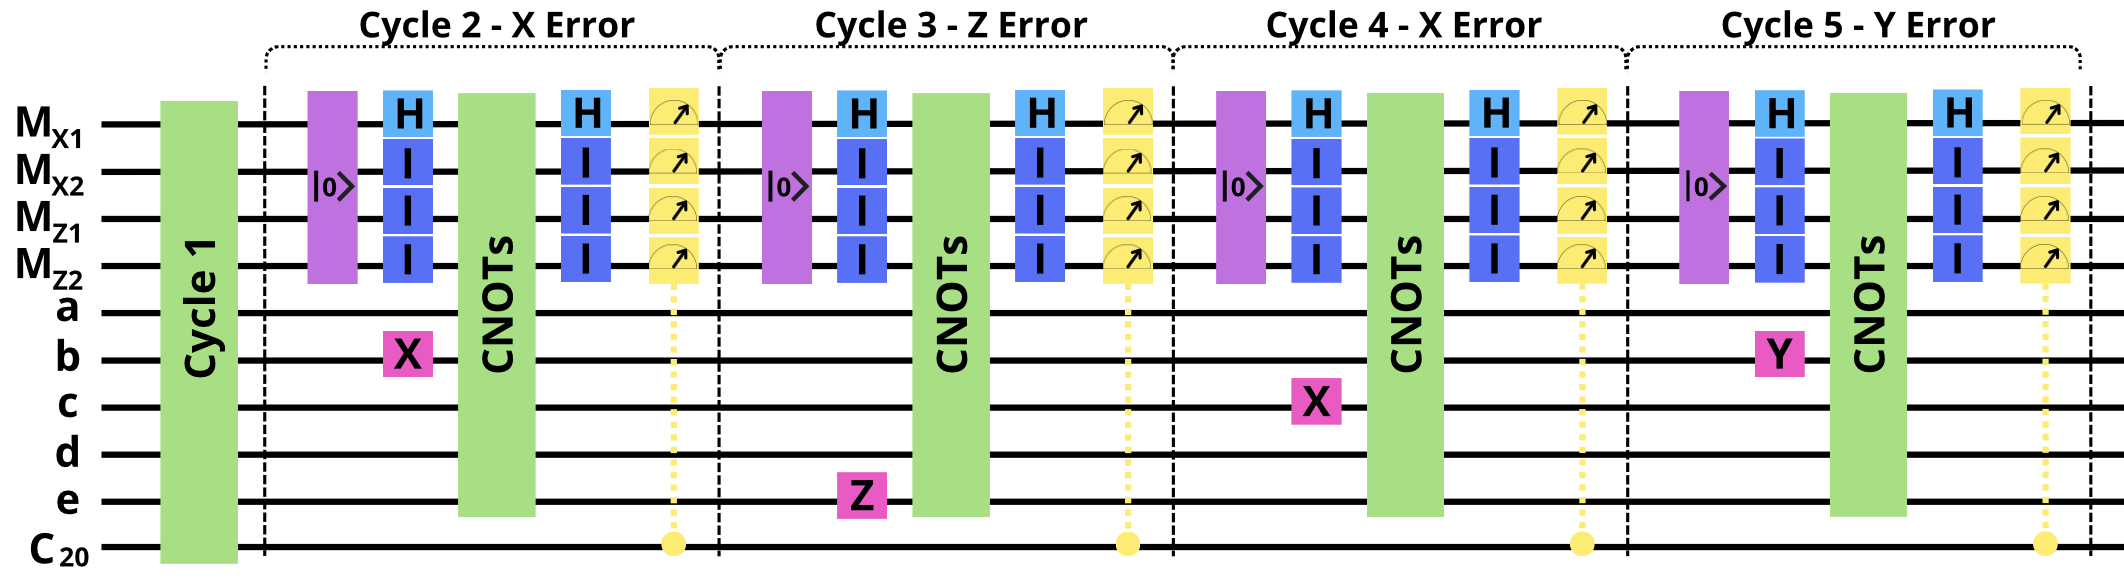
\includegraphics[width=1\linewidth]{figures/Circuit9qubitsErrors.png}
    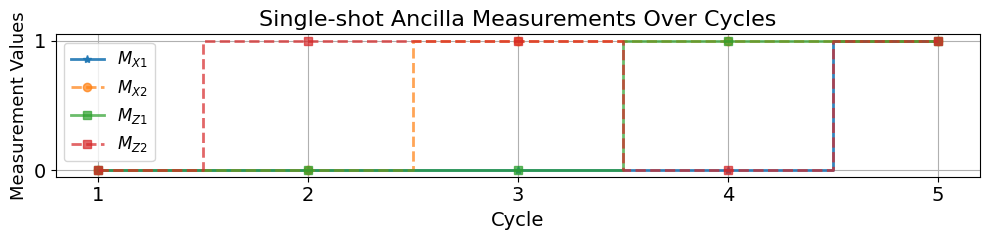
\includegraphics[width=1\linewidth]{figures/EigenvaulePlot9qubitsErrors.png}
    \caption{9-qubit Surface Code quantum circuit implementation over 5 cycles along with the stabilizer measurements effected by single qubit errors.}
    \label{fig:9qubit_eigenvlaues}
\end{figure}

 Errors were manually introduced at specific cycles to observe their effect on the stabilizer outcomes. In cycle 2, an \(X\) error on data qubit $Q_b$ flipped the eigenvalue of the \(Z\)-type stabilizer \(M_{Z2}\). During cycle 3, a \(Z\) error on qubit $Q_e$ flipped \(M_{X2}\). In the following cycle, an \(X\) error on qubit $Q_c$ caused \(M_{Z1}\) to flip to 1 and \(M_{Z2}\) back to 0 again. Finally, in cycle 5, a \(Y\) error on qubit $Q_b$ led to simultaneous flips of both \(M_{X1}\) and \(M_{Z2}\). Each stabilizer eigenvalue remaining flipped until impacted by a subsequent error on one of its connected data qubits. This behaviour confirms that the circuit correctly maps localized physical errors to changes in stabilizer outcomes, allowing for error detection in quantum codes.


\section{Noisy Gates for Simulating Quantum Computers} 
Accurate noise modeling is crucial for simulating quantum circuits in the NISQ\footnote{Noisy Intermediate-Scale Quantum (NISQ)} era, where quantum processors are still highly error-prone and classical simulations are key to understanding system behavior \cite{dibartolomeo2023noisy}. Traditionally, noise has been modeled by applying quantum channels before and after each ideal gate, effectively decoupling the noise from the gate operation itself. In contrast, Di Bartolomeo et al. proposes a new approach that integrates noise directly into the gate operation using the Lindblad formalism \cite{dibartolomeo2023noisy}. This method captures the full gate-and-environment dynamics by solving the Lindblad equation during the gate's execution, offering a more physically accurate simulation. The resulting “noisy gates” reproduce system behavior more realistically, without introducing additional computational cost compared to conventional methods.
This approximation only holds if the gate implementation $t_g$ is much shorter than the timescales over which the system interacts with its environment.

\subsection{Noise Implementation}
To model noise during quantum gate operations, we adopt the Lindblad formalism, which describes the non-unitary dynamics of open quantum systems under Markovian decoherence \cite{dibartolomeo2023noisy}. In the presence of noise, the evolution of the system can no longer be described by a purely unitary operator but must instead follow a Lindblad-type master equation. To move from the density matrix formalism to the state-vector picture, one applies a linear stochastic unraveling of the Lindblad equation, yielding an Itô stochastic differential equation for the state evolution \cite{dibartolomeo2023noisy}.
\begin{equation}
    d|\psi_s\rangle = \left[ -\frac{i}{\hbar} H_s ds + \sum_{k=1}^{N^2-1} \left( i \epsilon\, dW_{k,s} L_k - \frac{\epsilon^2}{2} ds\, L_k^\dagger L_k \right) \right] |\psi_s\rangle
    \label{eq:stochastic differential equation for modelling noisy quantum gates}
\end{equation}

where the $L_k$ are Lindblad operators, $dW_{k,s}$ are standard Wiener increments and $\epsilon \ll 1 $ is the noise strength. In the interaction picture, the Lindblad operators become time-dependent due to the coherent gate evolution and are written as:

\begin{equation}
    L_{k,s}=L_k(s) = U_s^\dagger \sigma_k U_s
    \label{eq: L_(k_s)}
\end{equation}

where $U_s$ is the unitary evolution operator generated by the applied gate. This unitary satisfies the Schrödinger equation $i\hbar \frac{dU_s}{ds} = H_s U_s$, with $U_{s=1} = U_g$ and $s \in [0,1]$ parametrizing the gate duration \cite{dibartolomeo2023noisy}.

Following the assumptions made by Di Bartolomeo et al, we consider single-qubit gates implemented on IBM’s superconducting devices, which take the form $U(\theta, \phi) = \exp(-i \theta R_{xy}(\phi)/2)$, where $R_{xy}(\phi) = \cos(\phi) X + \sin(\phi) Y$ defines the rotation axis in the XY-plane \cite{dibartolomeo2023noisy}. These gates are generated by the effective Hamiltonian.
\begin{equation}
    H(\theta, \phi) = \frac{\theta \hbar}{2} R_{xy}(\phi),
    \label{eq: H}
\end{equation}

applied over a unit time interval $s \in [0,1]$. While real hardware typically uses time-dependent shaped pulses $\omega_s$, we follow Di Bartolomeo in assuming constant pulse amplitude for simplicity \cite{dibartolomeo2023noisy}.

Averaging over the noise yields the density matrix $\rho_s = \mathbb{E}[|\psi_s\rangle\langle\psi_s|]$ (see Appendix \ref{appendix:Averaging over noise} for full proof), which satisfies the Lindblad master equation. The corresponding noisy gate $N_g$ at $s = 1$ can then be expressed as a product of deterministic and stochastic components:
\begin{equation}
N_g = U_g e^{\Lambda} e^{\tilde\Xi}
\label{eq: noisy gate N}
\end{equation}
with the deterministic operator $\Lambda$ and the stochastic components $\tilde{\Xi}$ and $\mathcal{C}$.
\begin{align}
\Lambda &= -\frac{\epsilon^2}{2} \int_0^1 ds \sum_{k=1}^{N^2-1}[L_{k,s}^\dagger L_{k,s} -L_{k,s}^2] \label{eq:lambda}\\
\tilde\Xi &= i\epsilon\sum_{k=1}^{N^2-1} \int_0^1 dW_{k,s}L_{k,s} + \mathcal{C} \label{eq:xi}\\
\mathcal{C} &= - \dfrac{\epsilon^2}{2} \sum_{k,l = 1}^{N^2-1}\int_0^1 dW_{k, s} \int_0^s dW_{l, s'} [L_{k,s}, L_{l,s'}] \label{eq:C_term}
\end{align}

However the \(\mathcal{C}\) term in~\eqref{eq:C_term} involves a nested Itô integral over adapted (non-anticipating) operator-valued functions. While this term is formally of order \(\epsilon^2\), its expectation vanishes due to the properties of Itô integrals. In particular, the following identities hold (See Appendix \ref{appendix:Itô calculus} for the full derivation):

\begin{equation}
    \mathbb{E}[dW_{k,s}] = 0\;, \quad \quad
    \mathbb{E}[dW_{k,s} \, dW_{l,s'}] = \delta_{kl} \delta(s - s')\, ds \label{eq:ito_isometry}
\end{equation}

As a result, for adapted integrands,

\begin{equation}
    \mathbb{E} \left[ \int_0^1 \int_0^s dW_{k,s} \, dW_{l,s'} \, [L_{k,s}, L_{l,s'}] \right] = 0
    \label{eq: expectation over ito integrals}
\end{equation}

This follows from the fact that the commutators \([L_{k,s}, L_{l,s'}]\) are non-anticipating and independent of future increments of the Wiener processes. Therefore, the contribution from \(\mathcal{C}\) vanishes under stochastic expectation, and the leading-order behavior of \(\Xi\) is given by the first-order Itô integral.
\begin{equation}
 \Xi = i\epsilon\sum_{k=1}^{N^2-1} \int_0^1 dW_{k,s}L_{k,s}
\label{eq: stochastic operator xi~}
\end{equation}

Despite the lack of norm preservation, averaging over noise recovers the correct physical behavior. An explicit expression for the noisy gate $N_g$ is obtained by expanding the evolution to second order in the small noise parameter $\epsilon$, yielding a perturbation to the ideal gate $U_g$. In the following subchapter, we derive the equations for the deterministic operator $\Lambda$ and the stochastic correction $\tilde{\Xi}$ that appear in this expansion, as given in Eq. ~\eqref{eq:lambda} - ~\eqref{eq:xi}.
 \newpage
\subsection{Perturbative Expansion in the Interaction Picture}
As a first step, we perform the stochastic unravelling in the interaction picture by defining the transformed state and time-ordered unitary evolution \cite{dibartolomeo2023noisy}.
\begin{equation}
    \ket{\phi_s} = U_s^\dagger \ket{\psi_s} \quad \text{where} \quad U_s = \mathcal{T} \exp\left( -\frac{i}{\hbar} \int_0^s H_\tau \, d\tau \right)
    \label{eq: transformed state in interaction picture}
\end{equation}

where \( H_\tau \) is the time-dependent system Hamiltonian and \(\mathcal{T}\) is the time-ordering operator required because \(H_{\tau}\) may not commute with itself at different times. This unitary operator generates the transformation to the interaction picture by removing the deterministic Hamiltonian evolution from the quantum trajectory \( \ket{\psi_s} \) \cite{dibartolomeo2023noisy}.
\begin{equation}
d \ket{\psi_s} = \left[ -\frac{i}{\hbar} H_s \, ds + \sum_k \left( i \epsilon L_k \, dW_{k,s} - \frac{\epsilon^2}{2} L_k^\dagger L_k \, ds \right) \right] \ket{\psi_s}
\label{eq: schrodinger_sde}
\end{equation}

To derive the interaction picture evolution, we apply the product rule:

\begin{equation}
    d\ket{\phi_s} = d(U_s^\dagger \ket{\psi_s}) = (dU_s^\dagger)\ket{\psi_s} + U_s^\dagger d\ket{\psi_s}
    \label{eq: d phi}
\end{equation}

Differentiating \( U_s^\dagger \), and noting that \( U_s \) satisfies
\begin{equation}
    \frac{d}{ds} U_s = \frac{-i}{\hbar} H_s U_s \quad \Rightarrow \quad \frac{d}{ds} U_s^\dagger = \frac{i}{\hbar} U_s^\dagger H_s \quad \Rightarrow \quad 
    dU_s^\dagger = \frac{i}{\hbar} U_s^\dagger H_s \, ds
    \label{eq: d U_s}
\end{equation}
we substitute into the expression for \( d\ket{\phi_s} \): 

\begin{equation}
d\ket{\phi_s} = \sum_k \left( i \epsilon \, dW_{k,s} \, U_s^\dagger L_k \ket{\psi_s} 
- \frac{\epsilon^2}{2} \, ds \, U_s^\dagger L_k^\dagger L_k \ket{\psi_s} \right)
\label{eq: d phi as sum}
\end{equation}

Using \( \ket{\psi_s} = U_s \ket{\phi_s} \), we rewrite the remaining terms as:
\begin{equation}
    U_s^\dagger L_k \ket{\psi_s} = U_s^\dagger L_k U_s \ket{\phi_s}, \quad 
U_s^\dagger L_k^\dagger L_k \ket{\psi_s} = (U_s^\dagger L_k^\dagger U_s)(U_s^\dagger L_k U_s) \ket{\phi_s}
\end{equation}

Defining the interaction-picture Lindblad operators as in Eq. ~\eqref{eq: L_(k_s)}, we obtain the Itô stochastic differential equation in the interaction picture \cite{dibartolomeo2023noisy}.
\begin{equation}
d\ket{\phi_s} = \left[ i \epsilon \sum_k dW_{k,s} L_{k,s} 
- \frac{\epsilon^2}{2} \sum_k ds \, L_{k,s}^\dagger L_{k,s} \right] \ket{\phi_s}.
\label{eq: stochastic unravelling in the interaction picture}
\end{equation}

To arrive at a usable form for simulating noisy gates, the gate evolution is discretized into $M$ infinitesimal time steps. Let $U_g$ denote the ideal (noiseless) gate. From the earlier formalism, we define the deterministic and stochastic contributions to the noisy evolution as:
\begin{equation}
    \Lambda = \frac{\epsilon^2}{2} A_m \quad \text{and} \quad \Xi = \epsilon B_m
    \label{eq: definition of A_m and B_m}
\end{equation}

where $A_m$ and $B_m$ correspond to the dissipative and stochastic effects respectively. Specifically, they are given by,
\begin{align}
    A_m &= -\frac{1}{M} \sum_{k=1}^{N^2-1} \left[ L_{k,m/M}^\dagger L_{k,m/M} - L_{k,m/M}^2 \right] \\
    B_m &= i \sum_{k=1}^{N^2-1} L_{k,m/M} \int_{m/M}^{(m+1)/M} dW_{k,m/M}
\end{align}

Here, $L_{k,m/M}$ are the interaction picture Lindblad operators evaluated at the discretized time slice $m/M$ \cite{dibartolomeo2023noisy}. \\
Given these definitions, the noisy gate over the entire duration can be expressed as the product:
\begin{equation}
    N_M = \prod_{m=0}^{M-1} e^{\Lambda + {\Xi}} = \prod_{m=0}^{M-1} e^{\epsilon B_m + \frac{\epsilon^2}{2} A_m}
    \label{eq: N_m expanded}
\end{equation}

This expression separates the noise dynamics from the ideal evolution $U_g$, allowing the full noisy gate to be expressed as 
\begin{equation}
    N_g = U_g \lim_{M \rightarrow \infty}  N_M
    \label{eq: N_M to infinity}
\end{equation}
Although it’s an approximation (accurate up to second order in $\epsilon$), it still gives a reliable and efficient way to simulate how noise affects the gate.

Applying the Baker-Campbell-Hausdorff formula\footnote{The Baker-Campbell-Hausdorff formula: 
\( \log(e^X e^Y) = X + Y + \frac{1}{2}[X,Y] + \frac{1}{12}[X,[X,Y]] + \frac{1}{12}[Y,[Y,X]] + \cdots \).} to 2nd order in $\epsilon$ to the product over $m$ in $N_M$ (from Eq. (\ref{eq: N_m expanded})) we obtain:
\begin{equation}
     N_M  = e^{\frac{\epsilon^2}{2} \sum_{m=0}^{M-1} A_m} e^{\epsilon \sum_{m=0}^{M-1} B_m}
     e^{ \frac{\epsilon^2}{2} \sum_{m=0}^{M-1} \sum_{n=0}^{k} [B_m, B_n] + \mathcal{O}(\epsilon^3)}
\end{equation}

At second order in $\epsilon$, the relevant terms are the cumulative sums of $\Lambda$ and $\Xi$, as well as the commutators between different $B_m$ operators.

We define the following shorthand expressions:
\begin{equation}
\mathcal{A}_M = \sum_{m=0}^{M-1} A_m, \quad 
\mathcal{B}_M = \sum_{m=0}^{M-1} B_m, \quad
\mathcal{C}_M = \sum_{m=0}^{M-1} \sum_{n=0}^{m} [B_m, B_n] 
\end{equation}
With these definitions, $N_M$ can be compactly written as:
\begin{equation}
     \label{eq: noisy gate N_M extended}
     N_M  = e^{\frac{\epsilon^2}{2} \mathcal{A}_M} e^{\epsilon \mathcal{B}_M + \frac{\epsilon^2}{2} \mathcal{C}_M + \mathcal{O}(\epsilon^3)}
\end{equation}

Taking the limit of $\mathcal{A}, \mathcal{B}$ and $\mathcal{C}$ separately we obtain a general form for N to the second order since it cannot be calculated analytically. 
\subsubsection*{Limit of $\mathcal{A_M}$}
We now define $\frac{1}{M} = ds$ and $s_m = \frac{m}{M}$, which lets us rewrite the discrete sum in $\mathcal{A}_M$ in terms of a Riemann sum:
\begin{equation}
    \mathcal{A}_M = -\frac{1}{M}\sum_{m=0}^{M-1} \sum_{k=1}^{N^2 - 1} \left[ L_{k,s_m}^\dagger L_{k,s_m} - L_{k,s_m}^2 \right]
\end{equation}

Taking the limit $M \to \infty$, the discrete sum becomes a Riemann integral\footnote{Riemann integral: 
\( \lim_{M \to \infty} \frac{1}{M} \sum_{m=0}^{M-1} f\left( \frac{m}{M} \right) = \int_0^1 f(s)\, ds \).} over the continuous variable $s \in [0,1]$.
\begin{equation}
    \lim_{M \to \infty} \mathcal{A}_M = - \sum_{k=1}^{N^2 - 1} \int_0^1 \left[ L_{k,s}^\dagger L_{k,s} - L_{k,s}^2 \right] \, ds
\end{equation}

\subsubsection*{Limit of $\mathcal{B_M}$}
We now turn to evaluating the limit of $\mathcal{B}_M$. Replacing the discrete label $m/M$ with a continuous variable $s_m$, this expression becomes
\begin{equation}
  \mathcal{B}_M = i \sum_{m=0}^{M-1} \sum_{k=1}^{N^2 - 1} L_{k, s_m} \int_{s_m}^{s_{m+1}} dW_{k,s_m}  
  \label{eq: B_M}
\end{equation}

In the limit \( M \to \infty \), the discrete sum over adjacent subintervals \( [s_m, s_{m+1}] \) converges to a continuous integral over the full interval \( [0,1] \), effectively transforming the sum into a Riemann–Stieltjes integral. Applying this to Eq.~\eqref{eq: B_M}, we obtain the continuum limit of \( \mathcal{B}_M \):
\begin{equation}
    \lim_{M \to \infty} \mathcal{B}_M = i \sum_{k=1}^{N^2 - 1} \int_0^1 L_{k,s} \, dW_{k,s}
\end{equation}


\subsubsection*{Limit of $\mathcal{C_M}$}
To compute the continuous-time limit of the commutator contributions to the noisy gate, we begin with the definition of the commutator between two stochastic terms $B_m$ and $B_n$. Specifically, the commutator is expressed as:
\begin{equation}
    [B_m, B_n] = - \left\{ \sum_{k,l}^{N^2 - 1} \int_{s_m}^{s_{m+1}} dW_{k,s_m} \int_{s_n}^{s_{n+1}} dW_{l, s_n} [L_{k, s_m}, L_{l, s_n}] \right\}
\end{equation}
The total correction term $\mathcal{C}_M$ then follows from summing these pairwise commutators
$
\mathcal{C}_M = \sum_{m=0}^{M-1} \sum_{n=0}^{m} [B_m, B_n],
$
which becomes
\begin{equation}
    \mathcal{C}_M = - \sum_{m=0}^{M-1} \sum_{n=0}^{m}\left\{ \sum_{k,l}^{N^2 - 1} \int_{s_m}^{s_{m+1}} dW_{k,s_m} \int_{s_n}^{s_{n+1}} dW_{l, s_n} [L_{k, s_m}, L_{l, s_n}] \right\}
\end{equation}
In the limit $M \to \infty$, the sums over the discrete subintervals $s_m = \frac{m}{M}$ converge to Riemann integrals over $s \in [0,1]$. We thus obtain the continuum limit of the second-order correction:
\begin{equation}
    \lim_{M \to \infty} \mathcal{C}_M = - \sum_{k,l}^{N^2-1} \int_0^1 dW_{k,s} \int_0^s dW_{l,s'} [L_{k,s}, L_{l,s'}]
\end{equation}
\subsubsection*{Putting Everything Together}

Now that each of the components $\Lambda$, $\Xi$, and $\mathcal{C}$ has been expressed in the continuum limit, we can combine them to recover the final expression for the noisy gate $N$ as stated in Eq.~\eqref{eq:lambda} - ~\eqref{eq:C_term}. These terms capture the respective deterministic dissipation, first-order stochastic fluctuations, and second-order stochastic correlations.
Substituting these into our expression for the noisy gate and taking the limit $M \to \infty$, we obtain:
\begin{equation}
    N = U_g \lim_{M \to \infty} N_M = U_g e^{\Lambda} e^{\Xi} e^{\mathcal{C}} = U_g e^{\Lambda} e^{\tilde{\Xi}}
\end{equation}
where the combined stochastic term $\tilde{\Xi}$ absorbs the full first-order and second-order contributions. 

\subsection{Depolarizing Noise Contribution}
To compute the full stochastic depolarizing contribution $\Xi(\theta, \phi)$ of the noisy gate, we begin by expressing each Lindblad operator $L_{k,s}$ as a linear combination of the Pauli basis $\{I, X, Y, Z\}$, which forms an orthonormal basis for single-qubit Hermitian operators. This decomposition takes the form:

\begin{equation}
    L_{k,s} = f_{k,s}^{(I)} I + f_{k,s}^{(X)} X + f_{k,s}^{(Y)} Y + f_{k,s}^{(Z)} Z = \left( \sum_{j=0}^{3} f_k^{(j)}(s) \sigma_j \right)
    \label{eq: L_k_s in pauli base}
\end{equation}
where the coefficients $f_k^{(j)}(s)$ are real-valued functions of time obtained by projection onto the corresponding Pauli elements:

\begin{equation}
    f_{k,s}^{(i)} = \frac{1}{2} \text{Tr} \left[ L_{k,s} \cdot \sigma_i \right]
    \label{eq: f as trace}
\end{equation}

Much like decomposing a vector in 3D space into its x, y, and z components, this allows us to fully reconstruct $L_{k,s}$ in terms of its action along each Pauli axis and track how noise evolves along distinct directions of the Bloch sphere. For the depolarizing channel specifically, the noise model is described by three time-dependent Lindblad operators:
\begin{equation}
L_{X,s} = \sqrt{\frac{p}{4}} \, X(s), \quad
L_{Y,s} = \sqrt{\frac{p}{4}} \, Y(s), \quad
L_{Z,s} = \sqrt{\frac{p}{4}} \, Z(s)
\end{equation}

where $p$ is the depolarizing probability. 

Substituting $L_{k,s}$ from Eq.~\eqref{eq: L_k_s in pauli base} into the definition of the stochastic gate, we write:
\begin{equation}
\begin{aligned}
    \Xi &= i\epsilon_d \sum_k \int_0^1 dW_{k,s} \, L_{k,s}
        = i\epsilon_d \sum_k \int_0^1 dW_{k,s} \left( \sum_{j=1}^{3} f_k^{(j)}(s) \sigma_j \right) \\
        &= i \epsilon_d \sum_{j=1}^{3}  \sum_k \left( \int_0^1 f_k^{(j)}(s) \, dW_{k,s} \right) \sigma_j
\end{aligned}
\label{eq:Xi_integral_expansion}
\end{equation}

Here, the parameter $\epsilon_d = \sqrt{\frac{p}{4}}$ represents the noise amplitude.
We then define a set of real stochastic variables (\( \xi_k^{(j)}\)) \cite{dibartolomeo2023noisy}:

\begin{equation}
   \xi_k^{(j)} = \int_0^1 f_k^{(j)}(s) dW_{k,s}
    \quad \rightarrow \quad
    \Xi = i \ \epsilon_d \sum_{j=1}^{3} \sum_k  \ \xi_k^{(j)}\  \sigma_j
    \label{eq: Xi as sum}
\end{equation}

This construction is particularly helpful because it isolates the stochastic influence in each Pauli direction, allowing us to identify how random fluctuations contribute to noise along the $X$, $Y$, and $Z$ axes independently. 
To fully characterize the distribution of $\Xi$, we compute the covariance matrix of the vector $\boldsymbol{\xi} = (\xi_x, \xi_y, \xi_z)$ \cite{dibartolomeo2023noisy}. The covariance matrix $\Sigma_{k}^{(ij)}$ expands to:

\begin{equation}
    \Sigma_{k}^{(ij)} = \mathbb{E}[\xi_k^{(i)} \xi_k^{(j)}] 
    \quad \rightarrow \quad 
    \Sigma_{k}^{(ij)} = \int_0^1 f_k^{(i)}(s) f_k^{(j)}(s) ds
    \label{eq: cov matrix}
\end{equation}

using Itô’s rule for Wiener processes, stated in Appendix \ref{appendix:Itô calculus}, Eq.~\eqref{eq:Wiener Function expecation}.

The full stochastic noise term $\Xi$ is constructed by decomposing it into contributions $\Xi_X$, $\Xi_Y$, and $\Xi_Z$ associated with each Pauli direction. Each of these components is computed by analyzing how the corresponding Pauli operator transforms under the unitary evolution $U_s$. Each conjugated operator is then decomposed in the Pauli basis: 
\begin{align}
    U_s^\dagger X U_s &= f_X^{(I)}(s)I +f_X^{(x)}(s) X + f_X^{(y)}(s) Y + f_X^{(z)}(s) Z\\
    U_s^\dagger Y U_s &= f_Y^{(I)}(s)I +f_Y^{(x)}(s) X + f_Y^{(y)}(s) Y + f_Y^{(z)}(s) Z\\
    U_s^\dagger Z U_s &= f_Z^{(I)}(s)I +f_Z^{(x)}(s) X + f_Z^{(y)}(s) Y + f_Z^{(z)}(s) Z
\end{align}

The coefficients $f_k^{(i)}(s)$ are obtained by evaluating Eq.~\eqref{eq: f as trace}. From these coefficients, we compute the corresponding stochastic variables $\xi_k^{(i)} = \int_0^1 f_k^{(i)}(s)\, dW_{k,s}$, which capture the effect of noise along each basis direction. 
The component $\Xi_k$ is then reconstructed as 
\begin{equation}
    \Xi_k = i\epsilon_d \sum_i \xi_k^{(i)} \sigma_i
    \label{eq: sum over xi components}
\end{equation}

and the total stochastic operator is obtained by summing over all Pauli components: 
\begin{equation}
    \Xi = \sum_k \Xi_k
\end{equation}
The full derivation and explicit expressions for components X,Y and Z are in Appendix \ref{appendix:Y Component}. 

\subsection{Amplitude Damping Contribution}
Amplitude damping noise is modeled via the Lindblad operator 
\begin{equation}
    L_{\downarrow,s} = \sqrt{\frac{1}{T_1}} \, \sigma_-(s)
    \label{eq: Lindbald Amplitude Damping}
\end{equation}

corresponding to the lowering operator $\sigma_- = \frac{1}{2}(X - iY)$, which captures energy relaxation from the excited to the ground state. $T_1$ is the relaxation time of the qubit. In the interaction picture, the time-evolved operator becomes 

\begin{equation}
    \sigma_-(s) = U_s^\dagger \sigma_- U_s = \frac{1}{2}(U_s^\dagger X U_s - i U_s^\dagger Y U_s)
    \label{eq: Lowering operator}
\end{equation}

This decomposition shows that $\sigma_-(s)$ is a linear combination of the same Pauli operators $X(s)$ and $Y(s)$ that appear in the depolarizing model, meaning the stochastic integrals used in both models are structurally identical. Specifically, the Itô integrals
\begin{equation}
    I_r^{(1)}=\int_0^1 dW_s, \quad I_r^{(2)}=\int_0^1 \sin(s\theta)\, dW_s, \quad I_r^{(3)}=\int_0^1 \sin^2(\frac{s\theta}{2})\, dW_s
\end{equation}
appear in both cases. 

These are used to construct a 3×3 multivariate Gaussian from which random samples are drawn and scaled by the amplitude damping factor \cite{dibartolomeo2023noisy}.
\begin{equation}
    \epsilon_1 = \sqrt{\frac{t_g}{T_1}}
\end{equation}
The stochastic contribution from dephasing noise is represented by the Hermitian matrix \cite{quantum_gates_repo}:
\begin{equation}
    \texttt{Ir} = \epsilon_1 \begin{pmatrix}
-\dfrac{i}{2} e^{i\phi} \, \text{I}_r^{(2)} & \text{I}_r^{(1)} - \text{I}_r^{(3)} \\
e^{2i\phi} \, \text{I}_r^{(3)} & \dfrac{i}{2} e^{i\phi} \, \text{I}_r^{(2)}
\end{pmatrix}
\end{equation}

\subsection{Phase Damping Contribution}
We also include the effect of dephasing noise, which primarily affects the phase coherence of the qubit without altering population. This noise is modeled using a Lindblad operator of the form 
\begin{equation}
    L_{Z,s} = \sqrt{\frac{1}{T_1}} \, Z(s)
\end{equation}

where $Z$ is the Pauli-Z operator. To compute its contribution in the interaction picture, we decompose the rotated $Z(s)$ operator into the Pauli basis $\{I, X, Y, Z\}$, and extract the associated real-valued functions $f_Z^{(i)}(s)$ for each Pauli component. These functions enter the second-order Itô expansion of the noise process, which determines the contribution to the covariance structure of the channel. Since this same procedure was already carried out in detail for the depolarizing noise contribution $\Xi$, we omit the intermediate steps here. The result is a $2 \times 2$ Hermitian matrix, denoted \texttt{Ip}, which captures the phase damping contribution \cite{quantum_gates_repo}.
\begin{equation}
    \texttt{Ip} = \epsilon_\phi \begin{pmatrix}
\text{I}_p^{(1)} & -i \, e^{-i\phi} \, \text{I}_p^{(2)} \\
i \, e^{i\phi} \, \text{I}_p^{(2)} & -\text{I}_p^{(1)}
\label{eq: Ip}
\end{pmatrix}
\end{equation}

The Itô-integrals $I_p^{(1)}$ and $I_p^{(2)}$ are equivalent to the Itô-integrals $I_Z^{(1)}$ and $I_Z^{(2)}$ for the Z component of the depolarizing noise (see Appendix \ref{appendix:Y Component}, Eq.~\eqref{eq: f_z}. 
This matrix is scaled by the effective dephasing amplitude \cite{dibartolomeo2023noisy}.
\begin{equation}
    \epsilon_\phi = \sqrt{\frac{1}{2} \left( \frac{t_g}{T_2} - \frac{t_g}{2T_1} \right)}
    \label{eq: e_psi}
\end{equation}

\subsection{Deterministic Noise Contribution}
In addition to stochastic fluctuations introduced by the environment, quantum operations are also subject to deterministic decoherence effects arising from the average behavior of the system-bath interaction \cite{Gu2019}. Within the Lindblad master equation formalism, these effects manifest as a Hermitian drift term that consistently biases the evolution of the system. In our model, the relevant jump operator $L_\downarrow(s)$ captures amplitude damping, representing energy loss through relaxation \cite{dibartolomeo2023noisy}. Unlike the stochastic component, which is inherently probabilistic and requires sampling over noise realizations, the deterministic term is computed directly and deterministically. Specifically, we construct the Hermitian operator $L_\downarrow^\dagger(s)L_\downarrow(s)$, integrate its matrix elements over time (from $s = 0$ to $1$), and extract three scalar functions \cite{quantum_gates_repo}. 
\begin{equation}
\text{det}_1 = \frac{\theta - \sin(\theta)}{2\theta}, \quad
\text{det}_2 = \frac{1 - \cos(\theta)}{\theta}, \quad
\text{det}_3 = \frac{\theta + \sin(\theta)}{2\theta}
\end{equation} 
corresponding to the integrated diagonal and off-diagonal contributions, with only the real-valued component of the off-diagonal retained \cite{dibartolomeo2023noisy}. This ensures that the deterministic matrix \(\Lambda\) remains Hermitian, consistent with the requirements of Itô calculus and quantum Lindblad evolution.
Finally, the deterministic matrix $\Lambda$ is assembled and contributes an exponential deformation $e^\Lambda$ to the gate.
\begin{equation}
    \Lambda = -\frac{\epsilon_1^2}{2} \begin{pmatrix}
\text{det}_1 & \frac{i}{2} e^{-i\phi} \text{det}_2 \\
-\frac{i}{2} e^{i\phi} \text{det}_2 & \text{det}_3
\end{pmatrix}
\end{equation}

\section{Noise Extension}
To apply this noise model in practice, we extended the implementation beyond what is available in the original library by Di Bartolomeo et al., who provide a Qiskit-compatible package for simulating noisy quantum gates\cite{dibartolomeo2023noisy,quantum_gates_repo}. Their implementation focuses exclusively on noise in the $R_{xy}$ direction, aligned with how physical gates behave on IBM quantum hardware. Specifically, IBM’s $Z$ gates are implemented virtually, meaning they introduce no additional noise \cite{mckay2017efficient}. As a result, the \textit{noisy-gates} library includes only noisy implementations for gates X, RY, SX, CX and ECR all modeled as subject to $R_{xy}$-type noise\cite{quantum_gates_repo}.

However, in our application, simulating a surface code, this limitation poses a problem. The surface code requires a noisy Hadamard gate, which is not a simple rotation in the XY plane. Since the Hadamard gate can be viewed as a combination of $X$ and $Z$ operations, we need to model noise on the $Z$ gate as well. To support this, we extended the noise model to general single-qubit rotations around arbitrary axes in the Bloch sphere. Specifically, we defined a generalized rotation axis 
\begin{equation}
    R_{xyz}(\phi, \psi) = \cos(\phi)\sin(\psi) X + \sin(\phi)\sin(\psi) Y +  \cos(\psi)Z
\end{equation}

and applied the corresponding unitary evolution $U = e^{-i\theta R_{xyz}/2}$. Using this formulation, we re-derived the expressions for the time-evolved Pauli operators $X(s)$, $Y(s)$, and $Z(s)$, computed their projections onto the Pauli basis, and constructed the associated covariance matrices. The resulting Itô integrals were sampled accordingly, and the updated analytic expressions are documented in Appendix \ref{appendix:Noise Extension}. While noise in the $R_{xy}$ model led to symmetric behavior between the $X$ and $Y$ components, the generalized $R_{xyz}$ noise introduces full rotational symmetry across all three Pauli directions.

Due to time constraints, we did not extend the $R_{xyz}$ noise model to two-qubit gates. However, this would be a natural and valuable direction for future work.

\subsection{Measurement Implementation}
Although the \texttt{noisy-gates} library provides gate-level noise modeling, it currently lacks mid-circuit measurement support; an important feature for accurately simulating surface codes and other measurement-based error-correction protocols\cite{quantum_gates_repo}.\\
To enable mid-circuit readout we implemented a custom measurement routine in QuTiP. For an \(N\)-qubit state \(\ket{\psi}\) and a target qubit \(i\), the code constructs the projectors:
\begin{align}
    P^{(i)}_{1} &= \bigl(I_{2}\bigr)^{\otimes i}\otimes\ket{1}\!\bra{1}\otimes\bigl(I_{2}\bigr)^{\otimes (N-i-1)} \\[4pt]
P^{(i)}_{0} &= \underbrace{\bigl(I_{2}\bigr)^{\otimes i}}_{\text{qubits }0\ldots i-1}
             \otimes\ket{0}\!\bra{0}
             \otimes\underbrace{\bigl(I_{2}\bigr)^{\otimes (N-i-1)}}_{\text{qubits }i+1\ldots N-1}
\end{align}

The Born-rule probabilities are then evaluated as
\begin{equation}
p_{0}= \bra{\psi} P^{(i)}_{0} \ket{\psi},
\qquad
p_{1}= \bra{\psi} P^{(i)}_{1} \ket{\psi},
\qquad
p_{0}+p_{1}=1
\tag{71}
\end{equation}

A measurement outcome \(k \in \{0,1\}\) is randomly selected based on the corresponding probabilities \(\{p_0, p_1\}\); the state is then collapsed according to the outcome, meaning it is projected onto \(P^{(i)}_k\) and re-normalized.

\begin{equation}
\ket{\psi_{out}} = 
\frac{P^{(i)}_{k}\,\ket{\psi}}{\sqrt{\bra{\psi}P^{(i)}_{k}\ket{\psi}}}
\tag{72}
\end{equation}

This updated state is fed back into the simulation, enabling measurements on any qubit at any point in the circuit.

\subsection{Noisy Reset Gate Implementation}
Since the \texttt{noisy-gates} library does not provide native support for noisy reset operations, an essential component in surface codes for repeated syndrome extraction, we implemented a custom reset procedure to incorporate realistic noise effects\cite{quantum_gates_repo}.

In our stochastic noise model, reset operations are implemented by performing a projective measurement on the target qubit, followed by a conditional application of a noisy \( X \) gate if the measurement outcome is \( |1\rangle \). 

\begin{figure}[H]
    \centering
    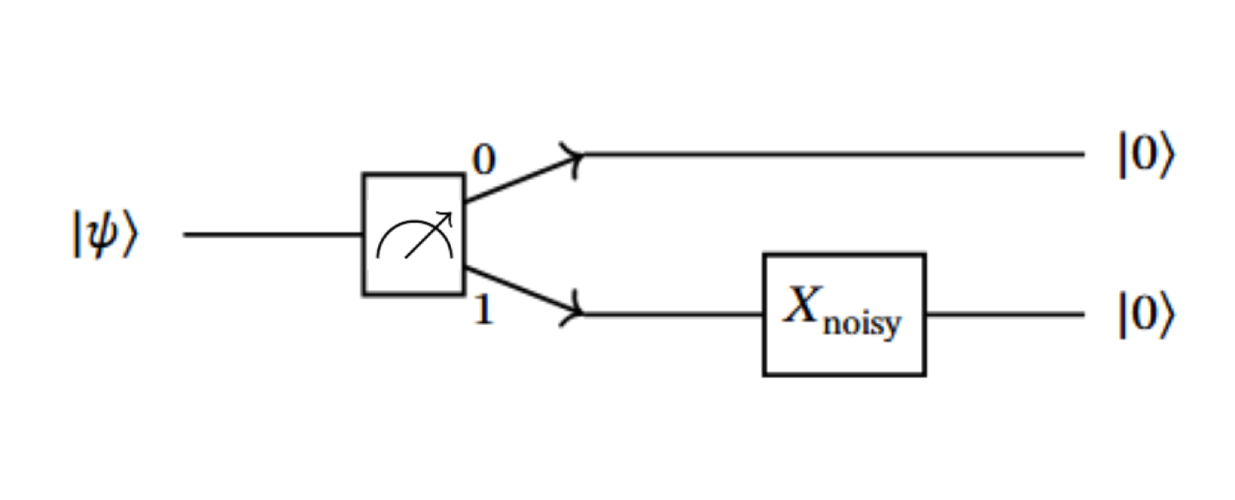
\includegraphics[width=0.35\textwidth, trim=0 120 0 120, clip]{figures/reset.jpg}
    \caption{Implementation of custom noisy reset gate.}
    \label{fig:trace_convergence}
\end{figure}

Specifically, the state is first collapsed via measurement, and if the result indicates an excited state, a stochastically generated noisy \( X \) gate, constructed using depolarizing, amplitude damping, and phase damping components is applied to return the qubit to \( |0\rangle \). This approach reflects a physically motivated, gate-based reset mechanism, as opposed to an idealized instantaneous projection to \( |0\rangle \).

\subsection{Noisy Hadamard Gate Implementation}

Since our framework applies noise individually to each gate, we construct the noisy Hadamard gate: \(H = \frac{1}{\sqrt{2}} \left[\begin{smallmatrix} 1 & 1 \\ 1 & -1 \end{smallmatrix}\right]\), by combining the noisy \( X \) and \( Z \) gates. The implementation is given by:

\begin{equation}
H_{\text{noisy}} = \frac{1}{\sqrt{2}}\left(X_{\text{noisy}} + Z_{\text{noisy}}\right)
\end{equation}

This approach is valid because the Hadamard gate can be represented as a balanced superposition of \( X \) and \( Z \).

\section{Results}

After computing the single-qubit gate noise components using the \( R_{xyz} \) decomposition, including depolarizing, amplitude damping, phase damping, and deterministic noise; these were integrated into the simulations of the four-qubit surface code. The code was implemented in QuTiP, enabling the non-unitary evolution required to simulate the stochastic noise model.
For all simulations and comparisons, the input state was initialized as:
\begin{equation}
|\psi_{\text{in}}\rangle = |0\rangle_{M_x} \otimes |\Phi^+\rangle_{D_a, D_b} \otimes |0\rangle_{M_z}
\end{equation}

Where the Bell state is defined as:

\begin{equation}
|\Phi^+\rangle_{D_a,D_b} = \frac{1}{\sqrt{2}} \left( |00\rangle + |11\rangle \right)_{D_a,D_b}
\end{equation}

This state preparation places the entangled pair on qubits $D_a$ and $D_b$, while qubits $M_x$ and $M_z$ are initialed to the computational $\ket{0}$ state. The Bell state's high sensitivity to decoherence and entanglement-breaking noise makes it a suitable probe for evaluating the impact of stochastic errors, particularly in detecting asymmetric or non-unitary contributions across the code.\\
To approximate realistic device behavior, noise parameters were extracted from the IBM Quantum backend \texttt{IBM Sherbrooke} using the \texttt{QiskitRuntimeService}. The extracted values include the amplitude damping time \( T_1 = 373~\mu\text{s} \), phase damping time \( T_2 = 336~\mu\text{s} \), single-qubit gate depolarizing error probability \textit{\( p = 2.31 \times 10^{-4} \)}, and average single-qubit gate duration \( t_g = 533~\text{ns} \). These parameters were used as the baseline for the simulations and informed the parameter sweeps, enabling analysis of realistic noise scenarios representative of single-qubit gate performance in a superconducting quantum processor.

\subsection{Analysis of Custom Noise Implementation}
\subsubsection*{Effect of Noise Model over on Measurement Outcomes}
To evaluate the effectiveness of our noise model, we analyzed the output distribution after one cycle of the four-qubit surface code. For the input state \( |\psi_{\text{in}}\rangle = |0\rangle_{M_x} \otimes |\Phi^+\rangle_{D_a, D_b} \otimes |0\rangle_{M_z} \), the only valid outcomes without noise are \( |0000\rangle \) and \( |0110\rangle \), each with equal probability. Under the influence of our stochastic noise model, particularly during Hadamard gate applications additional states such as \( |1000\rangle \) and \( |1110\rangle \) appear due to error-induced bit flips. The absence of patterns like $\ket{0001}$ or $\ket{0111}$ can be explained by the behavior of the noisy reset and the fact that the measurement qubits $M_x$ and $M_z$ are re-initialized to the ground state at the start of each cycle. Since no additional noise is applied to the $Z$ qubit and the reset measurement consistently returns 0, the conditional noisy $X$ gate is never triggered.
Fig.~\ref{fig:side_by_side_histograms} shows the resulting measurement distributions over 1000 shots for both realistic and amplified noise scenarios.
\begin{figure}[ht]
    \centering
    % Subfigure (a)
    \begin{subfigure}[b]{0.24\textwidth}
        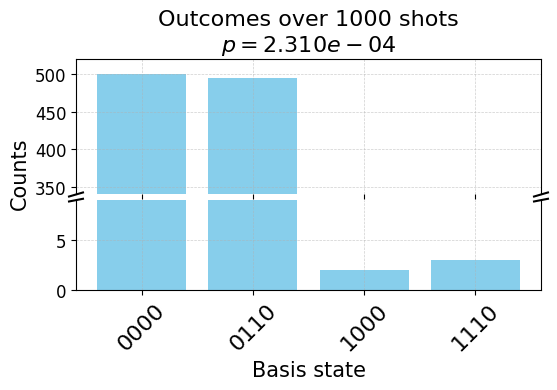
\includegraphics[width=\linewidth]{figures/new_counts_hist_p_real.png}
    \end{subfigure}
    \hfill
    % Subfigure (b)
    \begin{subfigure}[b]{0.24\textwidth}
        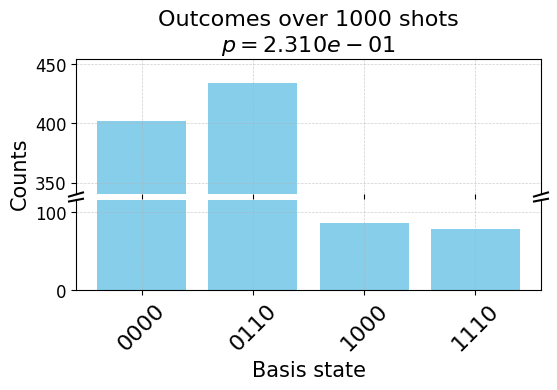
\includegraphics[width=\linewidth]{figures/new_counts_hist_p_1000x.png}
       \end{subfigure}
\vspace{-10pt} % Reduce space below
    \caption{Counts of Measurement outcomes (Left) Realistic noise level ($p$), (Right) Exaggerated noise \((1000 \times p)\).}
    \label{fig:side_by_side_histograms}
\end{figure}

Under realistic device noise, only about 5 total measurements correspond to erroneous states, whereas under exaggerated noise \( (10^3 \times p) \), the total count of noisy outcomes rises to \(~160\), indicating a significant increase in error rates driven by the stochastic noise model.
\subsubsection*{Single-Cycle Surface Code Behavior Under Realistic Noise}
To show the stochastic nature of our noise model, we analyzed the trace of the output state at each shot. For a general mixed state, the density matrix is given by
\begin{equation}
\rho = \sum_k p_k |\psi_k\rangle \langle \psi_k|, \quad \text{with} \quad \sum_k p_k = 1,
\end{equation}
where each \( p_k \) represents the probability of pure state \( |\psi_k\rangle \). The trace of \( \rho \) is then
\begin{equation}   
\mathrm{Tr}(\rho) = \sum_k p_k \, \mathrm{Tr}(|\psi_k\rangle \langle \psi_k|) = \sum_k p_k \langle \psi_k | \psi_k \rangle = \sum_k p_k = 1.
\end{equation}
This confirms that a properly normalized quantum state must have \( \mathrm{Tr}(\rho) = 1 \). In our stochastic simulation, however, each trajectory \( \rho_i = |\psi_i\rangle \langle \psi_i| \) arises from randomly sampled noise, and thus may not be individually normalized, i.e., \( \mathrm{Tr}(\rho_{noisy}) = \|\psi_{noisy}\|^2 \neq 1 \) in general. Nonetheless, the stochastic noise process is trace-preserving in expectation, so the average over many trajectories should converge to unity: \(\left\langle \mathrm{Tr}(\rho_i) \right\rangle \to 1.\)\\
We plotted the running mean of \( \mathrm{Tr}(\rho_i) \) with a root-mean-square error (RMSE) envelope to capture expected fluctuations, and included the absolute closeness to unity, defined as \( 1 - |\mathrm{Tr}(\rho_i) - 1| \), to quantify deviation from normalization. As shown in Fig.~\ref{fig:trace_convergence}, the running mean converges to 1 with minimal variance, consistent with the expected behavior of a trace-preserving noise process.
\begin{figure}[H]
    \centering
        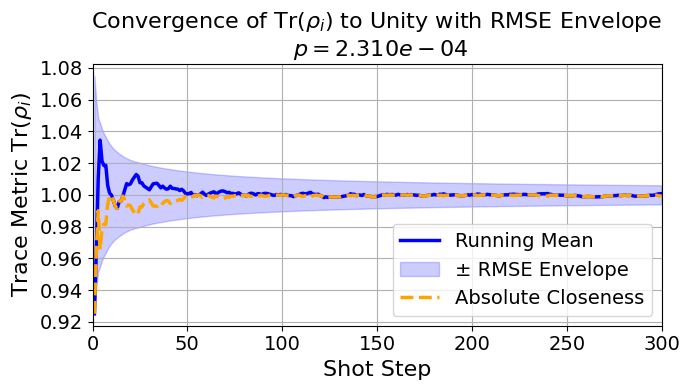
\includegraphics[width=1\linewidth]{figures/Trace_p_real_300.png}
        \caption{Running mean of trace convergence of \( \rho_i \) under realistic noise, with RMSE envelope, and absolute closeness to unity over 300 shots.}
    \label{fig:trace_convergence}
\end{figure}
We observe initial fluctuations in \( \mathrm{Tr}(\rho_i) \) ranging from approximately 0.92 to 1.04 for the first few shots, leading to a wide RMSE envelope that captures the variance in trace values. As the number of shots increases, both the envelope and the trace rapidly converge toward 1, along with the absolute closeness metric, demonstrating the expected averaging behavior of a trace-preserving stochastic process.\\
As seen in Fig.~\ref{fig:trace_convergence_worse}, amplifying the noise strength significantly increases the variance in the early trace values. 
\begin{figure}[H]
    \centering
        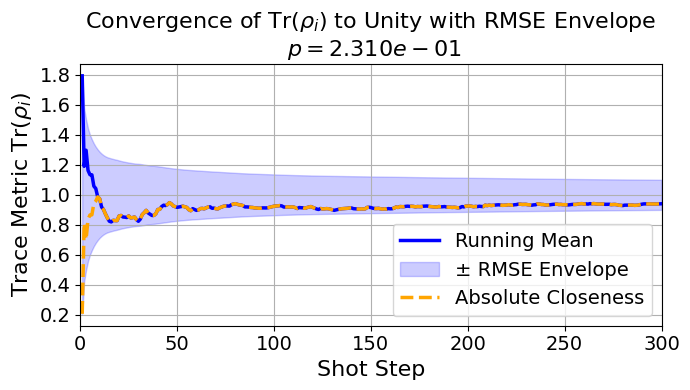
\includegraphics[width=1\linewidth]{figures/Trace_p_1000x_300.png}
    \caption{Running mean of trace convergence of \( \rho_i \) under exaggerated noise \((1000 \times p)\), with RMSE envelope, and absolute closeness to unity over 300 shots.}
    \label{fig:trace_convergence_worse}
\end{figure}
The running trace initially deviates by as much as 0.8 from unity and takes longer to stabilize; even after 300 shots, it remains close to 1 but does not fully converge, with a noticeably wider RMSE envelope reflecting greater variability introduced by stronger noise.


Another important metric for evaluating the impact of noise is the fidelity between the noisy output state and the expected ideal state. For each shot, we compute the fidelity between the noisy simulations output state and the ideal target state \( \rho_{\mathrm{ideal}} \) using the standard Uhlmann fidelity formula \cite{dibartolomeo2023noisy}. 
\begin{equation}
\mathcal{F}(\rho_i, \rho_{\mathrm{ideal}}) = \left( \mathrm{Tr} \sqrt{ \sqrt{\rho_{\mathrm{ideal}}} \rho_i \sqrt{\rho_{\mathrm{ideal}}} } \right)^2
\end{equation}
The ideal state \( \rho_{\mathrm{ideal}} \) corresponds to the expected output of the error-corrected surface code, which in this case is equivalent to the input state. We compute the running mean of the fidelity over successive shots to observe convergence behavior:
\begin{equation}
\langle \mathcal{F} \rangle_n = \frac{1}{n} \sum_{i=1}^n \mathcal{F}(\rho_i, \rho_{\mathrm{ideal}}),
\end{equation}
as well as the absolute closeness to unity, \( 1 - |\langle \mathcal{F} \rangle_n - 1| \), and the 95\% confidence interval using the standard error of the mean; as shown in Fig.~\ref{fig:fidelity_convergence_realistic}.

\begin{figure}[H]
    \centering
        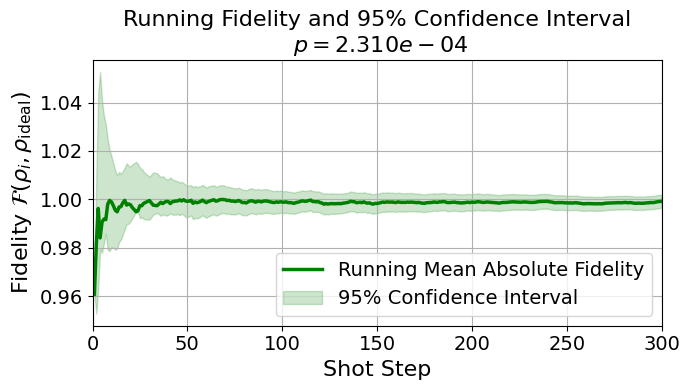
\includegraphics[width=0.5\textwidth]{figures/F_abs_p_real_300.png}
    \caption{Running absolute closeness of fidelity to unity, under realistic noise conditions along with confidence envelope of variance.}
    \label{fig:fidelity_convergence_realistic}
\end{figure}

Under realistic noise, the fidelity briefly deviates by up to 0.04 from unity, then rapidly stabilizes near 1 with tight confidence bounds, confirming consistent closeness to the ideal state. As shown in Fig.~\ref{fig:fidelity_convergence_worse}, increasing the noise level leads to a clear degradation in output fidelity.


\begin{figure}[H]
    \centering
        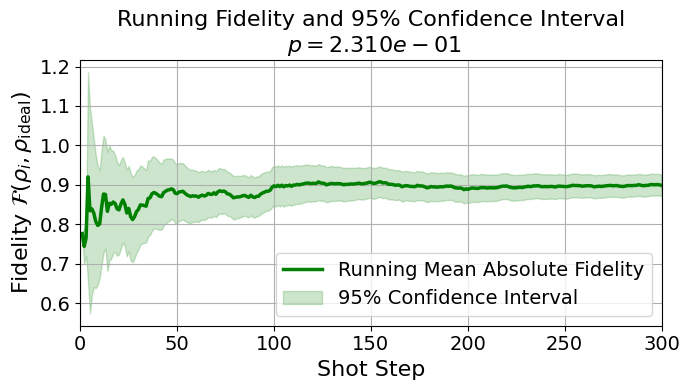
\includegraphics[width=0.5\textwidth]{figures/F_abs_p_1000x_300.png}
    \caption{Running absolute closeness of fidelity to unity, under heightened noise conditions \((1000 \times p)\) along with confidence envelope of variance.}
    \label{fig:fidelity_convergence_worse}
\end{figure}

In the exaggerated noise case, the fidelity initially deviates by more than 0.2 from unity, with a confidence envelope reaching up to 0.4 away from 1. Although the fidelity gradually improves over time, the running average converges only to approximately 0.9 after 300 shots, reflecting the impact of the amplified noise.\\
To visualize the impact of depolarizing noise on the output state, we performed a parameter sweep from \( p \times 10^{-1} \) to \( p \times 10^{6} \), tracking how both trace closeness and fidelity deviate from the ideal value of unity.

\begin{figure}[H]
    \centering
        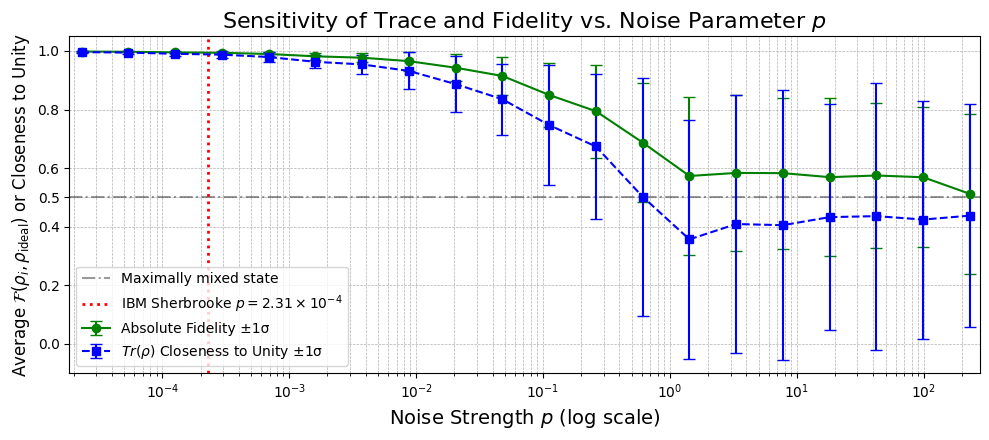
\includegraphics[width=1\linewidth]{figures/F_Trace_over_p.png} 
    \caption{Absolute closeness of fidelity and \(Tr(\rho)\) to unity over a sweep of depolarizing noise \(p\).}
    \label{fig:p_sweep_F_and_Tr}
\end{figure}

Fig.~\ref{fig:p_sweep_F_and_Tr} shows the average absolute fidelity and trace closeness to unity over 100 shots for 20 depolarizing noise values, with standard deviation error bars. Both metrics remain close to 1 for noise values near the device-calibrated level, then steadily decrease as \( p \) increases, until around \( \approx 1 \) (or \( 10^4 \times p \)). Beyond this point, the fidelity and trace converge toward 0.5, as expected for a maximally mixed state representing a completely random output. As noise increases, the error bars grow significantly, reflecting increased variability due to more uniform sampling across all possible output states under strong depolarization.


\subsection{Comparison to Qiskit Noise Simulation}
To compare with our custom stochastic noise model, we also implemented the four-qubit surface code in Qiskit using a standard noise model constructed from amplitude damping, phase damping, and depolarizing channels applied to the \texttt{X} and \texttt{H} gates, along with a Pauli error channel on \texttt{Reset}. This allows us to study how the output differs from stochastic evolution, which samples noise at the state level and may produce non-unit-trace intermediate states, unlike Qiskit's channel-based implementation that preserves trace at every step by construction. We expect small differences in output distributions and fidelity behavior due to these fundamental modeling distinctions.

\subsubsection*{Effect of Noise Model over Many Surface Code Cycles}
One can understand the effect of noise on the surface code over multiple cycles by analyzing the measurement outcomes of the \( X \)- and \( Z \)-type stabilizers, where an outcome of 0 indicates the expected (ideal) state and 1 signals a detected error. Fig.~\ref{fig:qiskit_traj_compare} shows the distribution of these stabilizer measurements over 20 surface code cycles using the Qiskit noise model.

\begin{figure}[H]
    \centering
    \begin{subfigure}[b]{\linewidth}
        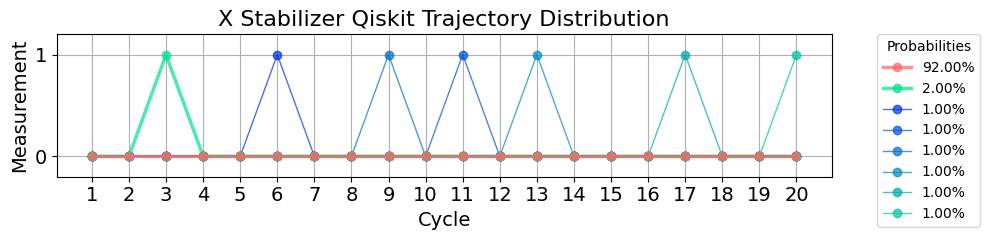
\includegraphics[width=\linewidth]{figures/qiskit_traj_X.png}  
    \end{subfigure}
    \hfill
    \begin{subfigure}[b]{\linewidth}
        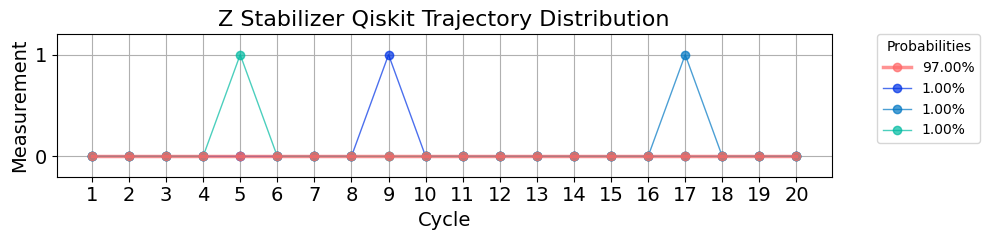
\includegraphics[width=\linewidth]{qiskit_traj_Z.png}        
    \end{subfigure}
    \caption{Comparison of X and Z stabilizer measurement trajectories from Qiskit simulation.}
    \label{fig:qiskit_traj_compare}
\end{figure}

The measurement outcomes are predominantly 0, consistent with expected behavior under low noise levels, while occasional 1s correspond to detected errors. These infrequent events reflect the underlying noise parameters and illustrate the stabilizers' role in capturing single-qubit errors over successive cycles.

As expected, the \( X \) stabilizer exhibits more errors, on average three times as many as the \( Z \) stabilizer, due to the presence of two Hadamard gates and one reset gate, whereas the \( Z \) stabilizer is only affected by the noisy reset operation. While our custom noise model produced similar results for the \( X \) stabilizer, it showed no errors in the \( Z \) stabilizer, as illustrated in Fig.~\ref{fig:traj_compare}.

\begin{figure}[H]
    \begin{subfigure}[b]{\linewidth}
        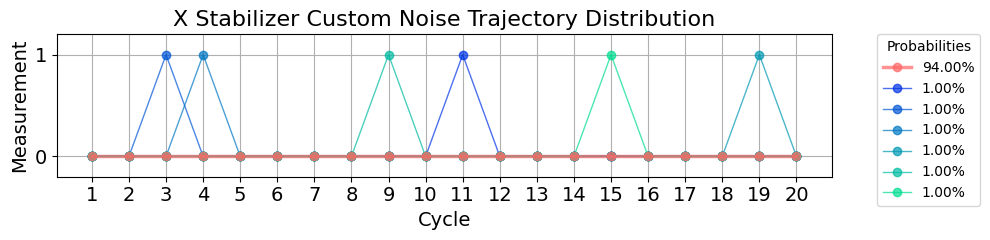
\includegraphics[width=\linewidth]{qutip_traj_X.png}
    \end{subfigure}
    \hfill
    \begin{subfigure}[b]{\linewidth}
        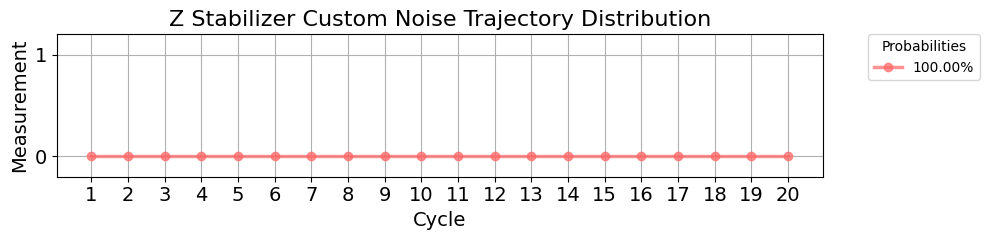
\includegraphics[width=\linewidth]{qutip_traj_Z.png} 
    \end{subfigure}
    \caption{Comparison of X and Z stabilizer measurement trajectories from  custom noise in QuTiP simulation.}
    \label{fig:traj_compare}
\end{figure}

This difference arises from a fundamental distinction in how the reset gate noise is modeled: in the Qiskit implementation, the reset gate includes a Kraus channel that applies noise regardless of the input state.  In contrast, our model applies a noisy \( X \) gate only when the measurement outcome is \( |1\rangle \). Since the input state is prepared noiseless and contains no \( |1\rangle \) component on the \( Z \) stabilizer qubits, no reset-induced noise is applied, consistent with how resets are typically performed in hardware, leaving the \( Z \) stabilizer unaffected. This setup was intentionally chosen to highlight the implementation difference between the two noise models.

\subsubsection*{Comparison of Noise Models on a Single Cycle Code}
To evaluate the impact of the two noise models on the input state over a single surface code cycle, we plot the average absolute fidelity over 500 shots, including standard deviation, as a function of the depolarizing noise strength.

\begin{figure}[H]
    \centering
        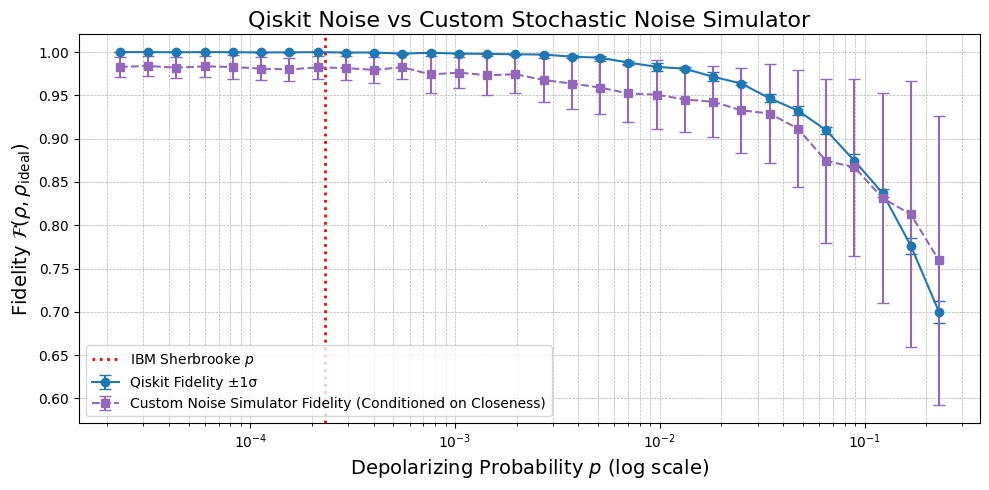
\includegraphics[width=1\linewidth]{figures/Fidelity_Qiskit_vs_Qutip.jpeg}
    \caption{Comparison of absolute fidelity of Qiskit noise model and stochastic noise model over a range of depolarizing noise strengths.}
    \label{fig:fidelity_comparison}
\end{figure}

As seen in Fig.~\ref{fig:fidelity_comparison}, the stochastic model yields absolute fidelities comparable to those of the Qiskit model across the full range of \( p \). The slightly lower fidelity in the stochastic model could be due to its inclusion of additional non-unitary noise contributions, specifically the deterministic noise, which are not present in the Qiskit implementation. Despite these differences, both models maintain high fidelity under realistic depolarizing noise levels. Compared to the Qiskit model, our stochastic noise model exhibits a significantly higher standard deviation in fidelity at large \( p \), which is expected due to the inherent variability introduced by sampling non-unitary stochastic noise.
To further quantify differences between the output states produced by the two noise models, we compute the Hellinger distance, defined as:

\begin{equation}
\mathcal{H}(\rho, \sigma) = \dfrac{1}{\sqrt{2}} \sqrt{\sum_{k=1}^N \left( \sqrt{\rho_{kk}} - \sqrt{\sigma_{kk}} \right)^2}
\end{equation}

Which measures the dissimilarity between two probability distributions based on their diagonal elements in the computational basis \cite{dibartolomeo2023noisy}. Unlike fidelity, which captures global state overlap, the Hellinger distance focuses on differences in measurement statistics, making it particularly useful for evaluating the practical impact of noise on observable outcomes \cite{dibartolomeo2023noisy}. As shown in Fig.~\ref{fig:hellinger_comparison}, we compute the Hellinger distance over a range of gate times \( t_g \), and plot the average over 500 shots including standard diviation of the stochastic model and Qiskit implmentation. Sweeping from \( 10^{-2} \times t_g \) to approximately \( 2 \times 10^3 t_g \).

\begin{figure}[H]
    \centering
        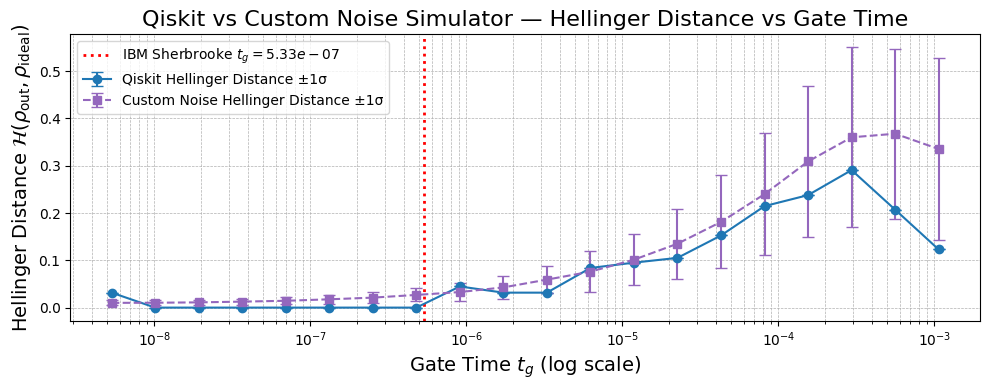
\includegraphics[width=1\linewidth]{figures/Hellinger_compare.png}
    \caption{Average Hellinger distance and standard deviation as a function of gate time \( t_g \), on Qiskit and custom stochastic noise models. Gate times range from \( 10^{-2} \times t_g \) to approximately \( 10^{3} \times t_g \)}
    \label{fig:hellinger_comparison}
\end{figure}

Across most of the gate-time sweep, the Hellinger distance from the custom stochastic model tracks the Qiskit result closely, especially near the hardware gate duration \( t_g \). Significant separation emerges only for very long gates (\( \sim 10^{3}\times t_g \)), and even then the Qiskit curve remains within the stochastic model’s \( \pm 1\sigma \) band. The consistently higher values obtained with the stochastic model can be attributed to the extra deterministic  noise included in that model but absent from the Qiskit configuration.\\
The stochastic noise model differs fundamentally from the Qiskit model in that it permits \emph{non-unitary} noise, whereas Qiskit remains strictly unitary.  
Fig.~\ref{fig:trace_comparison} highlights this distinction by sweeping the depolarizing probability over \(10^{-1}\times p_{\text{device}} \,\rightarrow\, 10^{3.2} \times p_{\text{device}}\) and plotting, for each value, the mean and standard–deviation error bars of the absolute trace-closeness to unity, averaged over 500 shots.

\begin{figure}[H]
    \centering
        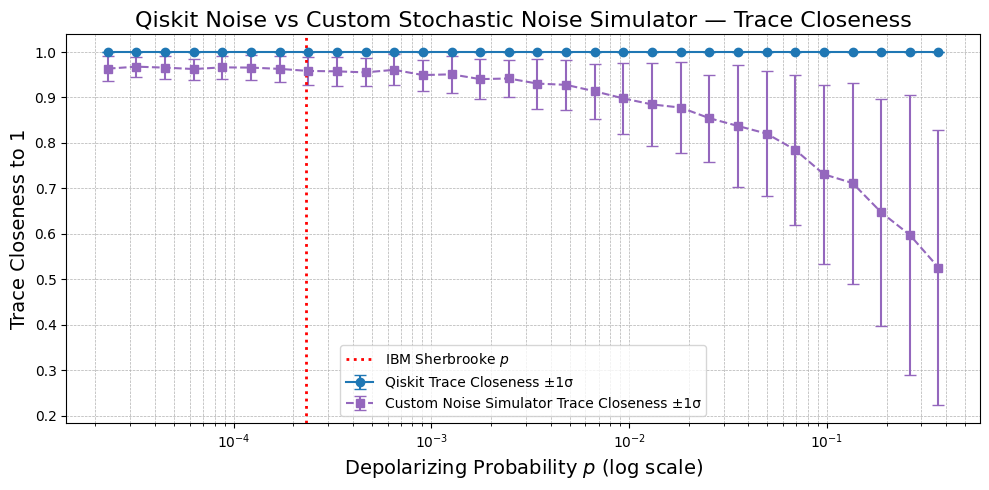
\includegraphics[width=1\linewidth]{figures/Trace_Qiskit_Qutip.png}
    \caption{Comparison of the trace closeness of the stochastic noise model to the Qiskit model as a function of the depolarizing probability \( p \).}
    \label{fig:trace_comparison}
\end{figure}

Fig.~\ref{fig:trace_comparison} shows that, as the depolarizing probability increases, the stochastic model evolves from an absolute \(\mathrm{Tr}(\rho)\) near unity toward, 0.5, the value expected for a maximally mixed state, while the Qiskit trace remains fixed at 1.  The accompanying growth in the stochastic model’s standard deviation reflects the larger shot-to-shot variability characteristic of realistic, non-unitary noise. In contrast, the Qiskit model applies a trace-preserving channel after every operation, forcing each trajectory to remain exactly normalized; this eliminates the population loss and variance observed in real hardware, making the model less representative of physical noise than the stochastic approach.
The results confirm that our generalized single-qubit noise matches Qiskit in fidelity and Hellinger distance, with trace non-preservation correctly reflecting non-unitary noise.

\section{Future Work}
Although this work has demonstrated the implementation of stochastic noise to single qubit gates on a 4-qubit surface code, there remain several promising directions for improvement and extension. These include both extensions to the surface code implementation and potentially expanding the capabilities of the \textit{noisy-gate} library.

\subsection*{Surface Code Extensions}
Because the current QuTiP implementation of noise and custom gates is fully modular to \(N\) qubits, extending the planar surface code from 4 to N qubits is straightforward. To achieve robustness against arbitrary single-qubit errors, the surface can be extended to a distance-3 code—requiring 17 qubits in a rotated layout (9 data + 8 ancilla) or 25 qubits in a non-rotated layout (13 data + 12 ancilla), as proposed by Fowler~\cite{fowler2012surface, fowler2014scalable}.

Introducing noise on two-qubit gates, however, is less trivial. Unlike single-qubit gates, which can often be decomposed into rotations and corrected with generic noise models, two-qubit gates such as the cross-resonance (CR) gate involve direct interaction terms that entangle multiple Hilbert subspaces. Future work will focus on developing physically motivated noisy two-qubit gate models that reflect these interactions.

Once two-qubit noise models are implemented, the full stochastic error model can be applied to a surface encoding a logical qubit. This will yield a minimally robust logical qubit that is first-order resilient to single-qubit errors.

With this noisy surface code in place, stabilizer measurement outcomes (syndrome streams) can be processed using Fowler’s implementation of Edmonds’ minimum-weight perfect-matching (MWPM) algorithm. This will enable us to evaluate how effectively the code maintains logical state coherence across multiple error-correction cycles under realistic noise.

Finally, once a full logical surface code, including single- and two-qubit gate noise, is implemented, we can compare our simulated performance directly against that of the same surface code run on real hardware, such as IBM Quantum devices. This enables a practical benchmark for how accurately the stochastic simulation captures the behavior of environmental noise in real quantum processors.

\subsection*{Potential Noisy Gates Library Improvements}
In addition to, or instead of, extending the surface code implementation, future work could enhance the capabilities of the \textit{noisy gates} library. 
One important improvement would be the addition of unit tests or error handling for unsupported circuit features, such as mid-circuit measurements, since current implementations do not issue warnings when incompatible components are used \cite{quantum_gates_repo}. 
Functionality for mid-circuit measurements could be introduced either via projective measurement sampling, as discussed in this work, or by decomposing circuits into sequential cycles evaluated with final measurements only. This framework could also support noisy reset gates, implemented conditionally based on mid-circuit outcomes. 
Further, the noise model could be generalized to arbitrary Hamiltonians by automating the computation of variance and covariance matrices, using symbolic sampling methods similar to those used for \(R_{xyz}\) component generation. Finally, the application and demonstration capabilities of the library could be expanded by including surface codes or other quantum error detection and correction schemes, showcasing the library's utility across a range of quantum computing algorithms \cite{quantum_gates_repo}.

\section{Conclusions}
The primary motivation behind this work was to implement single-qubit noise within a surface code framework, with the broader goal of aiding in the simulation and understanding of real quantum device noise and how it may be addressed using surface codes. We explore the theory of surface codes as presented by Fowler et al. \cite{fowler2012surface}, and the stabilizer formalism, along with the mechanisms of stochastic noise introduced by Di Bartolomeo et al. \cite{dibartolomeo2023noisy}, in order to fully understand how logical qubits can be protected against physical errors. 

Our implementation was guided by the surface code architecture introduced by Fowler, beginning with a 4-qubit layout and extending to a 9-qubit surface that includes stabilizer measurement circuits~\cite{fowler2012surface}. To model noise, we incorporated the physically motivated framework of Di Bartolomeo, which we further extended to handle general single-qubit rotations along arbitrary axes (\( R_{xyz} \))~\cite{dibartolomeo2023noisy}. In addition, we introduced support for mid-circuit measurements and noisy reset gates, enhancing the realism and versatility of the simulation environment. 

The resulting simulations produced outcomes consistent with Qiskit's noisy simulator for single-gate stochastic noise, validating the correctness of our model and implementation. Furthermore, we demonstrated that the full noisy operator approach, despite being non-unitary, offers promising paths for modeling physical decoherence processes and gate-specific noise, which cannot be captured by idealized Kraus channels alone.

This project offers a concrete step toward understanding how stochastic noise affects surface code performance, and sets the stage for deeper investigations into fault-tolerant quantum computing.

\section{Acknowledgments}
We would like to thank Professor Nicolas Macris and Perrine Vantalon for pointing us toward the foundational literature and for their time and helpful guidance throughout our work. We also thank the authors of the \textit{noisy gates} paper, in particular Michele Vischi, Roman Wixinger and Michele Grossi, for generously answering our technical questions via email. 
\newpage
\printbibliography
\newpage
% Insert appendix here
\appendix
\section*{\LARGE Appendix}

\section{Itô calculus}
\label{appendix:Itô calculus}

Let \( \{W_{k,s}\}_{k=1}^n \) denote a collection of independent Wiener processes (also known as standard Brownian motions), indexed by a discrete label \( k \) and continuous time \( s \geq 0 \).
Each process \( W_{k,s} = W_k(s)\) satisfies:

\begin{enumerate}
    \item \( W_{k,0} = 0 \)
    \item \( W_{k,s} \) has continuous sample paths
    \item The increments are independent and normally distributed: $W_{k,s+\Delta s} - W_{k,s} \sim \mathcal{N}(0, \Delta s)$
    \item The infinitesimal increment is denoted by \\\( dW_{k,s} := W_{k,s+ds} - W_{k,s} \)
\end{enumerate}

From 3. and 4. we can conclude \( dW_{k,s} := W_{k,s+ds} - W_{k,s} \sim \mathcal{N}(0, \Delta s) \)
\begin{align}
\mathbb{E}[dW_{k,s}] &= 0, \quad \mathbb{Var}[dW_{k,s}] = ds,\\
\mathbb{E}[dW_{k,s}^2] &= \mathbb{Var}[dW_{k,s}]+ (\mathbb{E}[dW_{k,s}])^2 = ds\\
\mathbb{E}[dW_{k,s} dW_{k',s}] &= \begin{cases} \mathbb{E}[dW_{k,s}]\mathbb{E}[dW_{k',s}],& \text{if } k\neq k', \\ \mathbb{E}[dW_{k,s}^2] = ds & \text{if } k = k' \end{cases} = \delta_{k,k'} \ ds
\label{eq:Wiener Function expecation}
\end{align}

Eq.~\eqref{eq:Wiener Function expecation} signifies that for \( k \ne k' \), the processes are independent \(\mathbb{E}[dW_{k,s} dW_{k',s}] = \delta_{k k'}\, ds\)

Another important identity is the Itô product rule: 

\begin{equation}
    d(XY) = dX \cdot Y + X \cdot dY + dX \cdot dY
    \label{eq: Itô product rule}
\end{equation}

\section{Averaging over noise}
\label{appendix:Averaging over noise}

We can rewrite Eq.~\eqref{eq:stochastic differential equation for modelling noisy quantum gates} as follows: 
\begin{align}
    d(\ket{\psi_s}) &= \bigg(\bigg[- \frac{i}{\hbar} H_s - \sum_{k=1}^{N^2-1}  \frac{\epsilon^2}{2} L_k^\dagger L_k \bigg]ds + \sum_{k=1}^{N^2-1}i\epsilon L_k d W_{k,s} \bigg)\ket{\psi_s} \notag\\
    &= \bigg(Ads + \sum_{k=1}^{N^2-1} B_k dW_{k,s} \bigg)\ket{\psi_s} \\
    d(\bra{\psi_s}) &= \bra{\psi_s} A^\dagger ds + \sum_{k'=1}^{N^2-1} \bra{\psi_s} B_{k'}^\dagger dW_{k',s}
\end{align}

For $A = [- \frac{i}{\hbar} H_s - \sum_{k=1}^{N^2-1}  \frac{\epsilon^2}{2} L_k^\dagger L_k \bigg]$ and $B_k = i\epsilon L_k$.\\
To describe the evolution of the system's density matrix in terms of stochastic pure states, we consider the stochastic unraveling of the Lindblad equation. Specifically, we define \( \rho_s = |\psi_s\rangle\langle\psi_s| \) as the pure state projector at time \( s \), and derive the evolution of the ensemble-averaged state \( \rho_t = \mathbb{E}[\rho_s] \). The following calculation shows how the master equation for \( \rho_t \) arises from the Itô stochastic differential equation governing \( |\psi_s\rangle \).

\begin{align}
    d(\ket{\psi_s}\bra{\psi_s}) &= d(\ket{\psi_s}) \bra{\psi_s} + \ket{\psi_s} d(\bra{\psi_s}) + d(\ket{\psi_s}) d(\bra{\psi_s})
    \label{eq: using Itô product rule}
\end{align}

Eq.~\eqref{eq: using Itô product rule} is obtained by applying the Itô product rule given in Eq.~\eqref{eq: Itô product rule} to the projector \( \rho_s = \ket{\psi_s} \bra{\psi_s} \).
\begin{equation}
d(\ket{\psi_s}) \bra{\psi_s} 
= \left(A \, ds + \sum_k B_k\, dW_{k,s}\right)\, \rho_s
\label{eq:diff1}
\end{equation}

\begin{equation}
\ket{\psi_s} d(\bra{\psi_s}) 
= \rho_s \left(A^\dagger \, ds + \sum_{k'} B^\dagger_{k'}\, dW_{k',s}\right)
\label{eq:diff2}
\end{equation}

\begin{align}
    d(\ket{\psi_s}) d(\bra{\psi_s}) &= \big(A\ ds+\sum_k B_kdW_{k,s}\big)\ \rho_s \ \big(A^\dagger ds+\sum_{k'} B^\dagger_{k'} dW_{k',s}\big) \notag \\
    &= A\ \rho_s \ A^\dagger d^2s + A \ \rho_s \sum_{k'} B_{k'} \ ds \ dW_{k',s} \notag\\ &+ \sum_{k} B_k \ \rho_s A^\dagger \ ds \ dW_{k,s} + \sum_{k,k'} B_k \ \rho_s B^\dagger_{k'} \ dW_{k,s}\ dW_{k',s} \label{eq: Itô correction term}
\end{align}



Among the terms in the expansion of Eq.~\eqref{eq: Itô correction term}, the product $A \ \rho_s \ A^\dagger ds^2$ arises. However, this term is of order $\mathcal{O}(ds^2)$ and can be neglected in the Itô calculus framework, which systematically retains terms only up to first order in the time increment $ds$. 

This neglect is justified by the fact that in the limit $ds \to 0$, terms proportional to $ds^2$ vanish faster than those linear in $ds$, and thus do not contribute to the stochastic differential equation's dynamics. More generally, in Itô calculus:

\begin{equation}
    \mathcal{O}(ds^2) \ll \mathcal{O}(ds) \quad \text{as} \quad ds \to 0,
\end{equation}

and therefore terms like $A \rho_t A^\dagger ds^2$ are discarded.
Accordingly, we retain only terms up to $\mathcal{O}(ds)$ in the expression for $d(\rho_s)$. 

To derive the evolution of the averaged state \( \rho_t = \mathbb{E}[\rho_s] \), we now take the expectation of both sides of Eq.~\eqref{eq: using Itô product rule}. As shown in Eq.~\eqref{eq:Wiener Function expecation}, the expectation of all terms involving a single stochastic increment \( dW_{k,s} \) or \( dW_{k',s} \) vanishes. The only non-zero stochastic contribution arises from the Itô correction term involving \( dW_{k,s} dW_{k',s} \), which satisfies $\mathbb{E}[dW_{k,s} dW_{k',s}] = \delta_{kk'}\, ds.$

Consequently, the double sum over \( k \) and \( k' \) in the final line of Eq.~\eqref{eq: Itô correction term} reduces to a single sum over \( k \). We obtain the following expression for the averaged state $\mathbb{E}[d(\rho_s)]$:

\begin{equation}
    \mathbb{E}[d(\rho_s)] = [A \ \rho_s + \rho_s A^\dagger + \sum_k B_k \ \rho_s \ B_k^\dagger] ds
    \label{eq: average over pure state}
\end{equation}
We now express the time derivative of the averaged state \( \rho_t \) by relating it to the derivative of the expectation value \( \mathbb{E}[\rho_s] \). Since differentiation and expectation commute, we obtain:

\begin{equation}
    \frac{d}{dt}\rho_t = \frac{d}{ds} \mathbb{E}[\rho_s] = \mathbb{E}[\frac{d}{ds} \ \rho_s] = A \ \rho_s + \rho_s A^\dagger + \sum_k B_k \ \rho_s \ B_k^\dagger = \mathcal{L}(\rho_s) 
\end{equation}

Integrating both sides of the above equation from \( 0 \) to \( t \) yields the formal solution for \( \rho_s \) in terms of the initial state \( \rho_0 \). Here, \( \mathcal{L} \) denotes the Lindbladian superoperator that generates the open-system dynamics.

\begin{equation}
    \rho_t = \int_0^t \frac{d}{ds} \rho_s \ ds + \rho_0 = \int_0^t \mathcal{L}(p_s) \ ds + \rho_0 = e^{t\mathcal{L}(p_s)}\rho_0
    \label{eq: averaged state}
\end{equation}

To justify the exponential form in Eq.~\eqref{eq: averaged state}, we expand the solution recursively by applying the integral equation iteratively. 
For a general first-order linear differential equation of the form

\begin{equation}
    \frac{d}{dt} X(t) = M(t) X(t),
\quad \rightarrow \quad 
X(t) = X(0) + \int_0^t M(s) X(s) \, ds,
\end{equation}

which motivates an analogous treatment for the evolution of the averaged density matrix \( \rho_t \).\\
In our case, the generator of the evolution is the Lindbladian superoperator \( \mathcal{L} \), which acts on an operator \( \rho \) according to

\begin{equation}
\mathcal{L}(\rho) = A \rho + \rho A^\dagger + \sum_{k} B_k \rho B_k^\dagger,
\label{eq: Lindbladian definition}
\end{equation}
where \( A \) and \( B_k \) are operator-valued coefficients derived from the system Hamiltonian and dissipative noise channels, respectively.

Since \( \mathcal{L} \) is linear and time-independent, we can write:
\begin{equation}
    \rho_t = \rho_0 + \int_0^t \mathcal{L}(\rho_s) \, ds.
    \label{eq: integral form}
\end{equation}

We now substitute Eq.~\eqref{eq: integral form} into itself to generate a Volterra-type expansion:
\begin{align}
    \rho_t &= \rho_0 + \int_0^t \mathcal{L} \left( \rho_0 + \int_0^s \mathcal{L}(\rho_u) \, du \right) ds \notag \\
           &= \rho_0 + \int_0^t \mathcal{L}(\rho_0) \, ds + \int_0^t \int_0^s \mathcal{L}^2(\rho_u) \, du \, ds \notag \\
           &= \rho_0 + t \mathcal{L}(\rho_0) + \frac{t^2}{2!} \mathcal{L}^2(\rho_0) + \cdots,
\end{align}

where we relabel the integration variables and iteratively expand under the assumption of a time-independent \( \mathcal{L} \). 

This yields the Dyson-type series:
\begin{equation}
    \rho_t = \sum_{n=0}^\infty \frac{t^n}{n!} \mathcal{L}^n(\rho_0) = e^{t\mathcal{L}} \rho_0,
    \label{eq: exponential lindblad}
\end{equation}
which confirms the exponential representation in Eq.~\eqref{eq: averaged state}. 

\section{Explicit calculation of the depolarizing component}
\label{appendix:Y Component}

\subsection{Y Component}
We consider the general $U_s$ for a $R_{xy}(\theta,\phi)$ rotation.
Therefore, the conjugation of the $Y$ Pauli operator is $Y(s) = U_s^\dagger Y U_s$:

\begin{equation}
    U_s^\dagger Y U_s = \begin{pmatrix}
    -\sin(s\theta)\cos(\phi) & i(-\cos^2(\frac{s\theta}{2})+e^{-2i\phi} \sin^2(\frac{s\theta}{2})\\
    i(\cos^2(\frac{s\theta}{2})-e^{2i\phi} \sin^2(\frac{s\theta}{2}) & \sin(s\theta)\cos(\phi) 
\end{pmatrix}
\end{equation}

Each of the components is found by applying:  $f_{i,s}^{(Y)} = \frac{1}{2} Tr[Y(s) \cdot \sigma_i]$ 

\begin{align}
    f_Y^{(z)}(s) &= \frac{1}{2}Tr[Y(s) \cdot \sigma_z] \notag \\  &= \frac{1}{2}Tr\begin{pmatrix}
    -\sin(s\theta)\cos(\phi) & i(\cos^2(\frac{s\theta}{2})-e^{-2i\phi} \sin^2(\frac{s\theta}{2}) \\
    i(\cos^2(\frac{s\theta}{2})-e^{2i\phi} \sin^2(\frac{s\theta}{2}) & -\sin(s\theta)\cos(\phi) 
\end{pmatrix} \notag \\
    &= -\sin(s\theta)\cos(\phi) \ ,\\[1.5ex]
    f_Y^{(I)}(s) &= \frac{1}{2}Tr[Y(s) \cdot \sigma_z] = 0 \ ,\\
    f_Y^{(x)}(s) &= \sin(2\phi)\cdot \sin^2(\frac{s\theta}{2})\ ,\\
    f_Y^{(y)}(s) &= 1 + 2(1-\sin^2(\phi))\cdot \sin^2(\frac{s\theta}{2})
    \label{eq: f_Y}
\end{align}

From this we can compute $\xi_Y^{(j)} := \int_0^1 f_Y^{(j)}(s) dW_{k,s}$:
\begin{flalign}
    \xi_Y^{(I)} &= 0 \ , &&\\
    \xi_Y^{(x)} &= \sin(2\phi) \cdot\int_0^1 \sin^2(\frac{s\theta}{2}) dW_{k,s} \ 
    \label{eq: zeta_Y_0}
\end{flalign}

\begin{flalign}
    \xi_Y^{(y)} &=\int_0^1 1 \cdot dW_{k,s} + 2(1-\sin^2(\phi) )\cdot\int_0^1 \sin^2(\frac{s\theta}{2}) dW_{k,s} \ , \\
    \xi_Y^{(z)} &= -\cos(\phi) \cdot\int_0^1 \sin(s\theta) dW_{k,s}
    \label{eq: zeta_Y}
\end{flalign}

This leaves us with three different integrals over $dW_{k,s}$.
    \begin{align}
    I_Y^{(1)}(s) &= \int_0^1 1 \cdot dW_{k,s} \ , \label{eq: Ito_integral_Y_1}\\
    I_Y^{(2)}(s) &= \int_0^1 \sin(s\theta) dW_{k,s} \ , \\
    I_Y^{(3)}(s) &= \int_0^1 \sin^2(\frac{s\theta}{2}) dW_{k,s}
    \label{eq: Ito_integral_Y_3}
\end{align}

\begin{align}
    \rightarrow \ \xi_Y^{(I)} &= 0, \quad\quad\quad\quad\quad\quad\quad\quad\quad\quad\quad \xi_Y^{(x)} = \sin(2\phi) \cdot I_Y^{(3)} \\
    \rightarrow \ \xi_Y^{(y)} &=I_Y^{(1)} + 2(1-\sin^2(\phi) )I_Y^{(3)}, \quad\ \xi_Y^{(z)} = -\cos(\phi) I_Y^{(2)}
\end{align}

Having defined $\xi_Y^{i}$ for all $i\in\{I,x,y,z\}$, we can compute the Y-component of $\Xi$ in Eq.~\eqref{eq: sum over xi components}:
\begin{equation}
    \Xi_Y = i \ \epsilon_d \sum_{j=1}^3 \xi_Y^{j}\sigma_i = 
    \begin{pmatrix}
        -\cos(\phi) \cdot I_Y^{(2)}& 
        -i \cdot I_Y^{(1)} + \alpha_-(\phi) \cdot I_Y^{(3)}\\
        i \cdot I_Y^{(1)} + \alpha_+ (\phi) \cdot I_Y^{(3)}& \cos(\phi) \cdot I_Y^{(2)}
    \end{pmatrix}
    \label{depolariziong noise X}
\end{equation}
with $\alpha_\pm = [\sin(2\phi)\pm 2i(1-\sin^2(\phi))] = \pm i \ (e^{\mp 2i\phi}+1)$.

The Itô-integrals (\ref{eq: Ito_integral_Y_3}) are sampled over the covariance matrix, computed as in Eq.~\eqref{eq: cov matrix}. The covariance matrix for the Y component discussed here is as follows:

\begin{equation}
\Sigma =
\begin{pmatrix}
0 & 0 & 0 & 0 \\
0 & \frac{2\theta - \sin(2\theta)}{4\theta} & \frac{\sin^4(\theta/2)}{\theta} & \frac{1 - \cos(\theta)}{\theta} \\
0 & \frac{\sin^4(\theta/2)}{\theta} & \frac{6\theta - 8\sin(\theta) + \sin(2\theta)}{16\theta} & \frac{\theta - \sin(\theta)}{2\theta} \\
0 & \frac{1 - \cos(\theta)}{\theta} & \frac{\theta - \sin(\theta)}{2\theta} & 1
\end{pmatrix}
\label{eq: Cov matrix Y}
\end{equation}

\subsection{X Component}
Although the $X(s)$ and $Y(s)$ components follow different time evolutions, they are both rotated under the same unitary family $U_s = e^{is\theta R_{xy}(\phi)}$, and the associated stochastic processes project onto the same set of underlying Itô integrals. This means that $X(s)$ and $Y(s)$ are driven by the same noise structure and thus share the same covariance matrix (\ref{eq: Cov matrix Y}). However, the functions $f_X^{(i)}(s)$ are not equal to $f_Y^{(i)}(s)$, as a result, the noise matrix $\Xi_X$ is constructed using the same integrals (\ref{eq: Ito_integral_Y_1}) - (\ref{eq: Ito_integral_Y_3}), but combined with distinct geometric prefactors specific to the $X$ axis:

\begin{equation}
    \Xi_X = \epsilon_d \begin{pmatrix}
\sin(\phi) \cdot \text{I}_X^{(2)}(s) & \text{I}_X^{(1)}(s) + (e^{-2i\phi} - 1) \cdot \text{I}_X^{(3)}(s) \\
\text{I}_X^{(1)}(s) + (e^{2i\phi} - 1) \cdot \text{I}_X^{(3)}(s) & -\sin(\phi) \cdot \text{I}_X^{(2)}(s)
\end{pmatrix}
\label{depolariziong noise X}
\end{equation} 
\subsection{Z Component}
We begin by computing the rotation of the Pauli-Z operator in the interaction picture under the unitary evolution \( U_s = e^{is\theta R_{xy}(\phi)} \). This gives:
\begin{equation}
        U_s^\dagger Z U_s = 
    \begin{pmatrix}
\cos(s\theta) & i(i\sin\phi - \cos\phi) \sin\left(s\theta\right) \\
(-\sin\phi + i\cos\phi) \sin\left(s\theta\right) & -\cos(s\theta)
\end{pmatrix}
\label{eq: UZU}
\end{equation}
To express this rotated operator in the Pauli basis, we extract its time-dependent coefficients, denoted \( f_Z^{(k)}(s) \), by projecting onto each Pauli matrix.

\begin{align}
f_Z^{(I)}(s) &= 0, \quad\quad\quad\quad\quad\quad\
f_Z^{(x)}(s) = -\sin(\phi)\sin(s\theta) \\
f_Z^{(y)}(s) &= \cos(\phi)\sin(s\theta), \quad 
f_Z^{(z)}(s) = \cos(s\theta), \\
I_Z^{(1)}(s) &= \int_0^1\ \sin(s\theta), \quad \;\;\;
I_Z^{(2)}(s) = \int_0^1 \ \cos(s\theta)
    \label{eq: f_z}
\end{align}

Using these basis functions, we build the noise contribution matrix \( \Xi_Z \) for the depolarizing channel, following the second-order stochastic model. This matrix includes the effect of rotation through the prefactor phase \( \phi \):

\begin{equation}
    \Xi_Z = \epsilon_d \begin{pmatrix}
I_Z^{(2)}(s) & -i \, e^{-i\phi} \, I_Z^{(1)}(s) \\
i \, e^{i\phi} \, I_Z^{(1)}(s) & -I_Z^{(2)}(s)
\end{pmatrix}
\end{equation}

Finally, the corresponding covariance matrix \( \Sigma \) for the stochastic noise contribution is computed by integrating the outer products of the Pauli basis coefficients \( f_Z^{(k)}(s) \). The result is a symmetric \(4 \times 4\) matrix that captures how the noise projects into each Pauli direction and their mutual correlations:

\begin{equation}
    \Sigma =
\begin{pmatrix}
0 & 0 & 0 & 0 \\
0 & \frac{(\theta - \sin(2\theta)/2)\sin^2(\phi)}{2\theta} & \frac{(-\theta + \sin(2\theta)/2)\sin(\phi)\cos(\phi)}{2\theta} & -\frac{\sin(\phi)\sin^2(\theta)}{2\theta} \\
0 & \frac{(-\theta + \sin(2\theta)/2)\sin(\phi)\cos(\phi)}{2\theta} & \frac{(\theta - \sin(2\theta)/2)\cos^2(\phi)}{2\theta} & \frac{\sin^2(\theta)\cos(\phi)}{2\theta} \\
0 & -\frac{\sin(\phi)\sin^2(\theta)}{2\theta} & \frac{\sin^2(\theta)\cos(\phi)}{2\theta} & \frac{\theta + \sin(2\theta)/2}{2\theta}
\end{pmatrix}
\end{equation}

\section{ Deterministic Term Contribution \( \Lambda \)}
Starting from noisy unitary evolution with small stochastic perturbations:

Drift (deterministic) term:

\begin{equation}
\Lambda(\rho) = -\frac{\epsilon^2}{2} \int_0^1 \sum_k \left[ L_{k,s}^\dagger L_{k,s} \rho + \rho L_{k,s}^\dagger L_{k,s} \right] ds
\end{equation}

In superoperator (operator-only) form:

\begin{equation}
\Lambda \approx -\frac{\epsilon^2}{2} \int_0^1 ds \sum_k L_{k,s}^\dagger L_{k,s}
\end{equation}

The term \( L_{k,s}^2 \) vanishes due to:

\begin{equation}
\mathbb{E}[L_{k,s}^2] = \mathbb{E}[(dW_{k,s})^2] L_k^2 = 0
\end{equation}

Thus, the reduced deterministic contribution is:

\begin{equation}
\Lambda = -\frac{\epsilon^2}{2} \int_0^1 ds \sum_k L_{k,s}^\dagger L_{k,s}
\end{equation}

\end{document}


\section{Noise Extension to $R_{xyz}$}
\label{appendix:Noise Extension}

\subsubsection*{Pauli Basis Components \( f_X^{(j)}(s) \) for \( R_{xyz} \) Rotation}
\begin{align*}
f_X^{(I)}(s) &= 0 \\
f_X^{(x)}(s) &= \sin^2(\psi) \sin^2\left( \tfrac{s\theta}{2} \right) \cos(2\phi)
- \sin^2\left( \tfrac{s\theta}{2} \right) \cos^2(\psi) + \cos^2\left( \tfrac{s\theta}{2} \right) \\
f_X^{(y)}(s) &= \sin(2\phi) \sin^2(\psi) \sin^2\left( \tfrac{s\theta}{2} \right)
- \sin(s\theta) \cos(\psi) \\
f_X^{(z)}(s) &= 2\left( \sin(\phi) \cos\left( \tfrac{s\theta}{2} \right)
+ \sin\left( \tfrac{s\theta}{2} \right) \cos(\phi) \cos(\psi) \right)
\sin(\psi) \sin\left( \tfrac{s\theta}{2} \right)
\end{align*}

\subsubsection*{Pauli Basis Components \( f_Y^{(j)}(s) \) for \( R_{xyz} \) Rotation}
\begin{align*}
f_Y^{(I)}(s) &= 0 \\
f_Y^{(x)}(s) &= \sin(2\phi) \sin^2(\psi) \sin^2\left( \tfrac{s\theta}{2} \right) + \sin(s\theta) \cos(\psi) \\
f_Y^{(y)}(s) &= -\sin^2(\psi) \sin^2\left( \tfrac{s\theta}{2} \right) \cos(2\phi)
- \sin^2\left( \tfrac{s\theta}{2} \right) \cos^2(\psi) + \cos^2\left( \tfrac{s\theta}{2} \right) \\
f_Y^{(z)}(s) &= 2\left( \sin(\phi) \sin\left( \tfrac{s\theta}{2} \right) \cos(\psi) 
- \cos(\phi) \cos\left( \tfrac{s\theta}{2} \right)\right) \sin(\psi) \sin\left( \tfrac{s\theta}{2} \right) 
\end{align*}

\subsubsection*{Pauli Basis Components \( f_Z^{(j)}(s) \) for \( R_{xyz} \) Rotation}

\begin{align*}
f_Z^{(I)}(s) &= 0 \\
f_Z^{(x)}(s) &= 2\left(-\sin(\phi) \cos\left( \tfrac{s\theta}{2} \right)
+ \sin\left( \tfrac{s\theta}{2} \right) \cos(\phi) \cos(\psi)\right)\sin(\psi) \sin\left( \tfrac{s\theta}{2} \right)
\end{align*}
\begin{align*}
f_Z^{(y)}(s) &= 2\left(\sin(\phi) \sin\left( \tfrac{s\theta}{2} \right) \cos(\psi)
+ \cos(\phi) \cos\left( \tfrac{s\theta}{2} \right) \right) \sin(\psi) \sin\left( \tfrac{s\theta}{2} \right) \\
f_Z^{(z)}(s) &= -2 \sin^2(\psi) \sin^2\left( \tfrac{s\theta}{2} \right) + 1
\end{align*}

In principle, the noise model based on rotation around a general axis $R_{xyz}$ allows for arbitrary unitary gates. However, calculating noisy gate dynamics in this fully general 3D setting quickly becomes analytically intractable due to the complexity of the operator evolution and resulting integrals. For this reason, we restrict our analysis to specific fixed-angle cases that correspond to actual quantum gates used in the surface code. As shown in Table \ref{table:angles}, we select concrete values for the rotation parameters $\phi$ and $\psi$ such that the noiseless part of the evolution $U_s = e^{-is\theta R_{xyz}(\phi, \psi)}$ implements a well-defined gate ($X$, $Y$, $Z$). For instance, to model a noisy $X$ gate, we choose $\phi = 0$ and $\psi = \pi/2$. By computing the noisy evolution only for such gates, we reduce computational overhead while still capturing all relevant behaviors of the noise model for fault-tolerant code simulations. \\
For the identity gate, \( \theta \) is fixed at \( 2\pi \), meaning there is no sampling over the rotation angle. As a result, no noise is introduced on \( I \), and the evolution remains perfectly noiseless.
\\

\begin{table}[h!]
\centering
\renewcommand{\arraystretch}{1.4}
\begin{tabular}{c c c c}
\toprule
\textbf{Gate} & \( \theta \) & \( \psi \) & \( \phi \) \\
\midrule
\( I \) & \( 2\pi \) & -- & -- \\
\( X \) & -- & \( \frac{\pi}{2} \) & 0 \\
\( Y \) & -- & \( \frac{\pi}{2} \) & \( \frac{\pi}{2} \) \\
\( Z \) & -- & 0 & \( \frac{\pi}{2} \) \\
\bottomrule
\end{tabular}
\caption{Rotation parameters \( (\theta, \psi, \phi) \) used to realize gates via $R_{xyz}(\phi,\psi)$.}
\label{table:angles}
\end{table}

\subsection{Demonstrating Rotational Symmetry in the Noise Model}
To illustrate the rotational symmetry of the depolarizing noise model, we examine the covariance matrices for noisy \( X \), \( Y \), and \( Z \) gates, each evaluated in its respective dominant component. In the \( X \) component of the noisy \( X \) gate, the variance is exactly 1, while all other components vanish; the same holds for the \( Y \) component of the noisy \( Y \) gate and the \( Z \) component of the noisy \( Z \) gate. This yields the following covariance matrices:

\begin{align*}
\text{Cov}_{X} &= 
\begin{pmatrix}
1 & 0 & 0 \\
0 & 0 & 0 \\
0 & 0 & 0
\end{pmatrix}, \quad
\text{Cov}_{Y} = 
\begin{pmatrix}
0 & 0 & 0 \\
0 & 1 & 0 \\
0 & 0 & 0
\end{pmatrix}, \quad
\text{Cov}_{Z} = 
\begin{pmatrix}
0 & 0 & 0 \\
0 & 0 & 0 \\
0 & 0 & 1
\end{pmatrix}
\end{align*}

These matrices clearly show that the noise distribution is symmetric under coordinate rotation: each principal axis is treated identically under depolarization.

In contrast the covariance matrices for the other directions (i.e., projecting a noisy \( X \) gate onto \( Y \) or \( Z \), etc.) contain non-trivial trigonometric structures of $\theta$. Below we list the corresponding Hermitian covariance matrices for the noisy Y gate when evaluated in the X and Z components.

\begin{equation}
\Sigma_Y^{(x)} =
\begin{pmatrix}
\frac{2\theta + \sin(2\theta)}{4\theta} & 0 & \frac{\sin^2(\theta)}{2\theta} \\
0 & 0 & 0 \\
\frac{\sin^2(\theta)}{2\theta} & 0 & \frac{2\theta - \sin(2\theta)}{4\theta}
\end{pmatrix}, \quad 
    \Sigma_Y^{(z)} =
\begin{pmatrix}
\frac{2\theta - \sin(2\theta)}{4\theta} & 0 & \frac{\sin^2(\theta)}{2\theta} \\
0 & 0 & 0 \\
\frac{\sin^2(\theta)}{2\theta} & 0 & \frac{2\theta + \sin(2\theta)}{4\theta}
\end{pmatrix}
\end{equation}

These matrices also exhibit a structural symmetry: the diagonal entries are symmetric combinations of \( 2\theta \pm \sin(2\theta) \), and the off-diagonal covariances involve \( \sin^2(\theta) \), always scaled by \( \theta \). This indicates that the model remains rotationally symmetric in structure. 

\section{Additional Figures}
\label{appendix:Additional Figures}
 \begin{figure}[H]
    \centering
        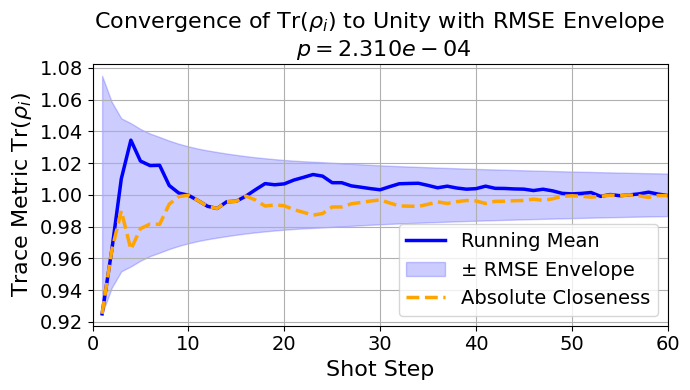
\includegraphics[width=1\linewidth]{figures/Trace_p_real_60.png}
    \caption{Comparison of X stabilizer measurement trajectories over 20 cycles for different simulators and decoders.}
    \label{fig:trajectories}
\end{figure}

\begin{figure}[H]
    \centering
        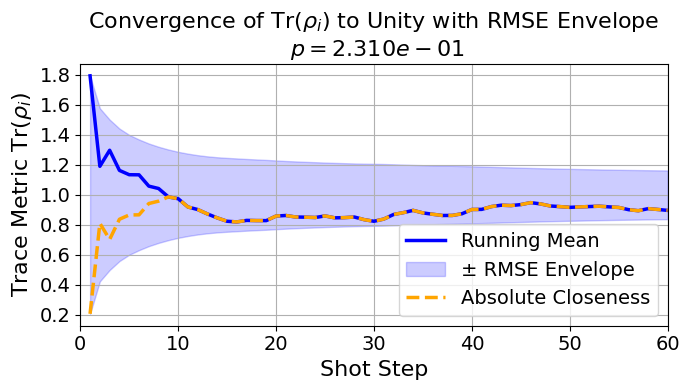
\includegraphics[width=1\linewidth]{figures/Trace_p_1000x_60.png}
    \caption{Comparison of X stabilizer measurement trajectories over 20 cycles for different simulators and decoders.}
    \label{fig:trajectories}
\end{figure}

\begin{figure}[H]
    \centering
        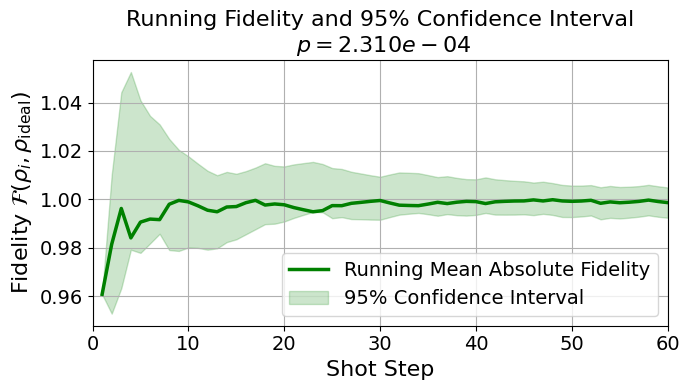
\includegraphics[width=1\linewidth]{figures/F_abs_p_real_60.png}
    \caption{Comparison of X stabilizer measurement trajectories over 20 cycles for different simulators and decoders.}
    \label{fig:trajectories}
\end{figure}

\begin{figure}[H]
    \centering
        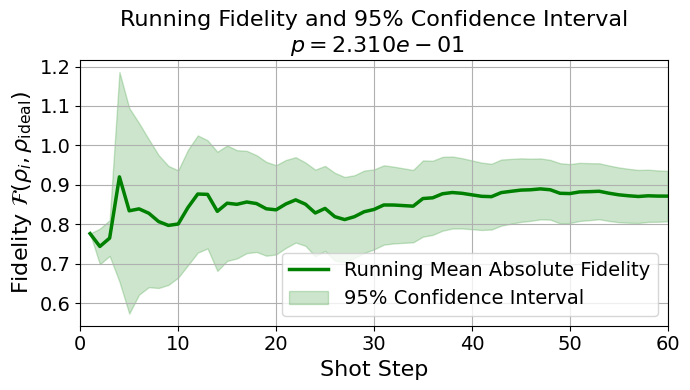
\includegraphics[width=1\linewidth]{figures/F_abs_p_1000x_60.png}
    \caption{Comparison of X stabilizer measurement trajectories over 20 cycles for different simulators and decoders.}
    \label{fig:trajectories}
\end{figure}

%----------------------------------------------------------




%----------------------------------------------------------

\end{document}